%%January 20- 2002
%\documentclass[wrr]{agu2001}
\documentclass{report}


\usepackage{natbibDK}
\usepackage{amsmath}
\usepackage{amssymb}
\usepackage[dvips]{graphicx}


\usepackage[T1]{fontenc}        %for danish letters
\usepackage[latin1]{inputenc}   %for danish letters


%%---------------------- For verification -----------------------------%%
\newcommand{\erf}{\operatorname{erf}}                   %new function names
\newcommand{\erfc}{\operatorname{erfc}}                 %new function names
\newcommand{\inverfc}{\operatorname{inverfc}}           %new function names
\newcommand{\inerfc}{\operatorname{i^nerfc}}            %repeated int of erfc
\newcommand{\imoneerfc}{\operatorname{i^{-1}efc}}       %repeated int erfc
\newcommand{\inmoneerfc}{\operatorname{i^{n-1}erfc}}
\newcommand{\izeroerfc}{\operatorname{i^0erfc}}
\newcommand{\ierfc}{\operatorname{ierfc}}
%%---------------------------------------------------------------------%%


\begin{document}

%% ------------------------------------------------------------------------ %%
%
%  TITLE
%
%% ------------------------------------------------------------------------ %%


\title{Formler til Milj\ostyrrelsen}

%% ------------------------------------------------------------------------ %%
%
%  AUTHORS AND AFFILIATIONS
%
%% ------------------------------------------------------------------------ %%

\author{Mikkel Mollerup}




\chapter{Water movement}


\section{Richards' Equation}

The water flow in porous media can be described with the formula of
Richard. The equation is derived here. The water flux density
vector, $\mathbf{q}$ can be calculated by the Darcy�s law. For a
two-dimensional vertical transect it yields:
\begin{equation}
\mathbf{q}=-\mathbf{K}(\psi)\nabla(\psi + z) \label{eq:darcy}
\end{equation}
where $\mathbf{K}(\psi)$ is the hydraulic conductivity tensor,
$\psi$ is the potential head. The x-axis is chosen in horizontal
direction and the z-axis is positive upwards. The conductivity
tensor can be expressed as:
\begin{equation}
\mathbf{K}=\begin{bmatrix} K_{xx} & K_{xz} \\ K_{zx} & K_{zz}
 \end{bmatrix}
\end{equation}
For a model with rectangular cells we have chosen that the
 principal directions of the anisotropic medium are parallel to
 the $x$- and $z$-axis, i.e.
\begin{equation}
\mathbf{K}=\begin{bmatrix} K_{xx} & 0 \\ 0 & K_{zz}
 \end{bmatrix}
\end{equation}
The mass balance for the system gives
\begin{equation}
\frac{\partial \theta}{\partial t}=-\nabla \cdot \mathbf{q}
-\Gamma \label{eq:continuity}
\end{equation}
where $\theta$ is the volumetric water content and $\Gamma$ is the
sink term. The partial differential equation can be developed by
combining Darcy�s law, equation \ref{eq:darcy} and the mass balance,
equation \ref{eq:continuity}, thus
\begin{equation}
\frac{\partial \theta}{\partial t}=\nabla \cdot
\left(\mathbf{K}(\psi)\nabla (\psi + z)\right) - \Gamma
\label{eq:richards}
\end{equation}
This is known as Richard's equation. For the modeling is assumed
that the soil-water retention is without hysteresis, i.e. there is a
unique relation between the matrix pressure potential and the water
content.

To solve Richard's equation it is necessary to specify initial and
boundary conditions. The boundary conditions specify a combination
of $\psi$ and its derivative on the boundary. Furthermore it is
possible to use different forms of flux (Neumann) and predescribed
pressure (Dirichlet) boundary conditions. The problem to be solved
for determining the water movement can be summarized to
%%% with moustages %%%
\begin{equation}
\begin{cases}
\frac{\partial \theta}{\partial t}=\nabla \cdot
\left(\mathbf{K}(\psi)\nabla (\psi + z) \right)-\Gamma & \text{in}\  \Omega \\
\mathbf{\bar{n}} \cdot \left(\mathbf{K}(\psi)\nabla (\psi + z)
\right)=
-q & \text{on}\ \partial \Omega^{N} \\
\psi=\psi_0 & \text{on}\ \partial \Omega^{D}
\end{cases}
\label{eq:watermovement}
\end{equation}
%%%%%%%%%%%%%%%%%%%%%%%
%%% without moustages %%%
%\begin{eqnarray}
%&& \frac{\partial \theta}{\partial t}=\nabla \cdot
%\left(\mathbf{K}(\psi)\nabla (\psi + z) \right)-\Gamma \ \text{in}\  \Omega  \nonumber \\
%&&\mathbf{\bar{n}} \cdot \left(\mathbf{K}(\psi)\nabla (\psi + z)
%\right)=
%-q \ \text{on}\ \partial \Omega^{N} \nonumber \\
%&&\psi=\psi_0 \ \text{on}\ \partial \Omega^{D}
%\label{eq:watermovement}
%\end{eqnarray}
%%%%%%%%%%%%%%%%%%%%%%%%%%
where $\mathbf{\bar{n}}$ is the outward unit normal, and $q$ is the
magnitude of the outward flow from the domain. $\psi_0$ is the
predescribed pressure at the boundary. $\Omega$ is the soil domain.
$\partial\Omega^{N}$ and $\partial\Omega^{D}$ are part of the
boundary of $\Omega$ with Neumann and Dirichlet boundaries,
respectively such that $\partial\Omega=\partial\Omega^{N} \cup
\partial\Omega^{D}$. Each of $\partial\Omega^{N}$ and
$\partial\Omega^{D}$ are not necessarily one continuous curve piece.
A special case of the Neumann boundary conditions is often applied
for the lower boundary condition, viz. it is assumed that the flow
it is only driven by gravity (gravity boundary condition), i.e.
$\partial \psi/
\partial x= \partial \psi/ \partial z=0$ which gives
\begin{equation}
q=\mathbf{\bar{n}} \cdot \begin{bmatrix}0 \\ K_{zz}
\end{bmatrix}
\end{equation}
Another often used boundary condition is the seepage boundary
condition for atmospheric boundaries. If a seepage face does not
develop, the boundary acts as no flow. If a seepage face occurs we
have a Dirichlet boundary condition with $\psi=0$ and allow water to
flow out of the domain. The condition can for instance be applied in
connection with estuaries or streams.



\section{Finite Volume Method}

\subsection{Mesh}

In Daisy2D, the domain, $\Omega$ is divided into $N$ non-overlapping
polygons, also denoted control volumes or cells. In Daisy2D it
should be possible to choose between grids consisting of only
rectangular cells or meshes consisting of trapezoids with two
vertical faces. Figure \ref{fig:grid_rect} shows a grid only
consisting of rectangular cells. The domain $\Omega$ in the figure
is in divided into 3 subdomains, each consisting of a number of
cells. Each subdomain is characterized by different hydraulic
properties. The grid shown in figure \ref{fig:grid_trapz} consists
of trapezoids (where most of them also are rectangles). Only in the
proximity of the drainpipe (see figure \ref{fig:grid_trapz_part}),
the cells are not rectangular.


\begin{figure}[h]
\includegraphics[width=\hsize]{grid_rect.eps}
\caption{Example of grid consisting of rectangular cells.}
\label{fig:grid_rect}
\end{figure}

\begin{figure}[h]
\includegraphics[width=\hsize]{grid_trapz.eps}
\caption{Example of grid consisting of trapezoids.}
\label{fig:grid_trapz}
\end{figure}

\begin{figure}[h]
\includegraphics[width=\hsize]{grid_trapz_part.eps}
\caption{Close picture of grid near the drain pipe.}
\label{fig:grid_trapz_part}
\end{figure}


The quadrilateral (rectangular or trapezoid) cells are denoted $Q_i$
where $i=1,2,\cdots, N$. $|Q_i|$ denotes the area of $Q_i$, and
$\partial Q_i$ is the boundary of $Q_i$ i.e. the edges (or faces) of
$Q_i$. All internal edges $e_{ij}$ are labeled by indices, $i$ and
$j$ of the adjacent cells that shares face. The grid is constructed
such that only whole faces are shared ($e_{ij}=Q_i \cap Q_j$). The
length of $e_{ij}$ is $|e_{ij}|$ and the unit normal vector pointing
from $Q_i $into $Q_j$ and orthogonal to $e_{ij}$ is denoted
$\bar{\mathbf{n}}_{ij}$. $\sigma_i$ contains cell indices of cells
sharing faces with cell $i$. $\sigma_i'$ contain indices of cell
faces of cell $i$ which are placed on $\partial \Omega$, i.e. it is
not shared with another cell.  $\sigma_i'$ is divided into two
subsets, $\sigma_{i}'^{D}$ and $\sigma_{i}'^{N}$ of boundary cell
faces with a Dirichlet and Neumann boundary condition, respectively.



\subsection{Cell mass-balances}

Richards equation is integrated over control volume (here a cell),
$Q_i$. By applying the divergence theorem by Green-Gauss, we
obtain
\begin{equation}
\int_{Q_i} \frac{\partial \theta}{\partial t} d \Omega =
\int_{\partial Q_i} \left(\mathbf{K}(\psi)\nabla (\psi + z)
\right)\cdot \mathbf{\bar{n}} dl - \int_{Q_i} \Gamma d\Omega
\label{eq:integratet}
\end{equation}
%
where $\mathbf{\bar{n}}$ is the outwarded unit normal and $\partial
Q_i$ the boundary of $Q_i$. The cell averages of $\theta$ and $\psi$
are denoted  $\theta_i$ and $\psi_i$. $\theta_i$ and $\psi_i$, $i=1,
2, \cdots N$ where $N$ is the number of cells that are collected in
the vectors $\boldsymbol{\theta}$ and $\boldsymbol{\psi}$.
Discretization  of equation \ref{eq:integratet} based on a grid
consisting of quadrilaterals yield

\begin{equation}
|Q_{i}|\frac{d \theta_i}{dt} = \sum_{j \in \sigma_i} D_{ij}(\boldsymbol{\psi})
 + \sum_{j \in \sigma_i} G_{ij}(\boldsymbol{\psi})
 + \sum_{j' \in \sigma_{i}'} B_{ij'}(\boldsymbol{\psi})
 - S_{i}(\boldsymbol{\psi})
\label{eq:discretised}
\end{equation}
%
where:

\begin{itemize}
\item $D_{ij}(\boldsymbol{\psi})$ describe the diffusive transport
between internal borders \item $G_{ij}(\boldsymbol{\psi})$
describe the gravitational transport between internal boundaries
\item $B_{ij'}(\boldsymbol{\psi})$ describe flux for external
boundaries $j'\in \sigma_{i}'$
\item $S_{i}(\boldsymbol{\psi})$ is the integrated sink term (point and area distributed sinks) in the cell. \\
\end{itemize}

The diffusive transport from cell $i$ to cell $j$ can be
calculated as

\begin{equation}
D_{ij}(\boldsymbol{\psi})=|e_{ij}|(\mathbf{K}(\boldsymbol{\psi})\cdot (\nabla \psi)_{ij})\cdot \mathbf{\bar{n}}_{ij}
\label{eq:diffusitive}
\end{equation}
%
For evaluating equation \ref{eq:diffusitive} it is necessary to
estimate the gradient $(\nabla \psi)_{ij}$. $(\nabla \psi)_{ij}$ is
evaluated by a different method for meshes with rectangular cells
than for the more general and complicated case with meshes
consisting of trapezoid cells. The gravitational transport from cell
$i$ to cell $j$ can be calculated as

\begin{equation}
G_{ij}(\boldsymbol{\psi})=|e_{ij}|(\mathbf{K}(\boldsymbol{\psi})\cdot([0\ 1]^T))\cdot \mathbf{\bar{n}}_{ij}
\label{eq:gravitational}
\end{equation}

The boundary flux term is split into the contribution from
boundaries with Neumann and Dirichlet condition respectively:

\begin{equation}
 \sum_{j' \in \sigma_{i}'} B_{ij'}(\boldsymbol{\psi}) = \sum_{j' \in \sigma_{i}'^N}
 B_{ij'}^{N}(\boldsymbol{\psi}) + \sum_{j' \in \sigma_{i}'^D} B_{ij'}^{D}(\boldsymbol{\psi})
\end{equation}
%
For the boundaries with Neumann conditions we have

\begin{equation}
B_{ij'}^{N}(\boldsymbol{\psi})= -q_{ij'}|e_{ij'}|
\end{equation}
%
where $q_{ij'}$ is the size of the Darcy flux, perpendicular to the
cell face and positive for flux out from cell $i$. The easiest way
to implement Dirichlet boundary conditions is simply to force
$\psi_i$ to the value that $\psi$ has on the face with Dirichlet
conditions. Conflicts can arise if cell $i$ has more than one face
with a Dirichlet condition. Instead, the Dirichlet boundary
condition is implemented as if the midpoint of the Dirichlet face
was a neighbor cell. Similar to an interior cell face, a diffusive
and a gravitational contribution can be calculated:

\begin{equation}
B_{ij'}^{D}(\boldsymbol{\psi}) = D_{ij'}^{D}(\boldsymbol{\psi}) +
G_{ij'}^{D}(\boldsymbol{\psi})
\end{equation}
%
where

\begin{eqnarray}
D_{ij'}^{D}(\boldsymbol{\psi})=|e_{ij'}|(\mathbf{K}(\psi_i)\cdot
(\nabla \psi)_{ij'})\cdot \mathbf{\bar{n}}_{ij'} \\
G_{ij'}^{D}(\boldsymbol{\psi})=|e_{ij'}|(\mathbf{K}(\psi_i)\cdot([0\
1]^T))\cdot \mathbf{\bar{n}}_{ij'}
\end{eqnarray}
%
where the pressure associated with cell $i$ has been used for
calculating the hydraulic conductivity. The sink term used in
equation \ref{eq:continuity} can be divided into two parts

\begin{equation}
\Gamma=\Gamma_A+\Gamma_p \delta(x_p-x)\delta(z_p-z)
\end{equation}
%
where $\Gamma_A$ is the contribution from a area distributed sink
and $\Gamma_P$ is the contribution from a point sink. $(x_p,z_p)$
are the coordinates of the point sink which shall be placed in the
interior of a cell(not on the cell faces). $\delta$ is the Dirac
delta function. Thus, the contribution from the sink terms to a cell
yields

\begin{equation}
S_{i}(\boldsymbol{\psi}) = \Gamma_A |Q_i| + \Gamma_P
\end{equation}
%
Area distributed sinks are typically extraction from roots or (in
Daisy2D) water flow between the soil matrix and macro pore domain.
The point sinks can be tile drains or drip irrigation systems (point
sources). Both $\Gamma_A$ and $\Gamma_P$ can be dependent on the
solution ($\psi$).



\subsection{Rectangular cells}

For the situation with a mesh consisting of rectangular cells, only
matrix pressure in the four neighbor cells (see figure
\ref{fig:meshrect_nswe}) are applied for calculating the fluxes
through the faces of the cell (five point stencil). In the present
section we will only evaluate the gradient for the "eastern" cell
face of cell $i$. The theory can easily be applied for the 3
remaining directions.
%
\begin{figure}[h]
\includegraphics[width=\hsize]{meshrect_nswe.eps}
\caption{Cell $i$ and the neighbor cells it share faces with.}
\label{fig:meshrect_nswe}
\end{figure}
%
The distances necessary for evaluating the flux from a cell to the
cell placed east of the cell are shown in figure
\ref{fig:meshrect_gradient}.

\begin{figure}
\includegraphics[width=\hsize]{meshrect_gradient.eps}
\caption{Distances used for calculation of flux between cell $i$
and its "eastern" neighbor.} \label{fig:meshrect_gradient}
\end{figure}

The value of $\psi$ in the midpoint of the eastern cell ($\psi_E$)
can be expressed by a Taylor expansion of the value of $\psi$ at
the midpoint of the cell face:

\begin{equation}
\psi_E = \psi(x+\delta x^+)=\sum_{k=0}^{m}  \frac{1}{k!} \left(\frac{d^k \psi}{dx^k}\right)_f (\delta x^+)^k  + R^+
\end{equation}
%
where $m$ is the order of the Taylor expansion and $R^+$ is the
Lagrange remainder. Similar can $\psi_i$ be computed

\begin{equation}
\psi_i = \psi(x-\delta x^-)=\sum_{k=0}^{m}  \frac{1}{k!} \left(\frac{d^k \psi}{dx^k}\right)_f (-\delta x^-)^k  + R^-
\end{equation}
%
It can be assumed that $R^+ - (-1)^{m+1}R^- \approx 0$. Thus if a
Taylor expansion of first order ($m=1$) is chosen we get

\begin{equation}
\left( \frac{d \psi}{dx} \right)_f (\delta x^+ +\delta x^-)\approx \psi_E-\psi_i
\end{equation}
%
If a higher order Taylor expansion is chosen we get

\begin{equation}
\left( \frac{d \psi}{dx} \right)_f (\delta x^+ +\delta x^-)\approx \psi_E-\psi_i - \epsilon_{Ei}
\end{equation}
%
where the correction term can be calculated as

\begin{equation}
\epsilon_{Ei} \approx \sum_{k=2}^{m}  \frac{1}{k!} \left(\frac{d^k
\psi}{dx^k}\right)_f \left[ (\delta x^+)^k - (-\delta x^-)^k \right]
\end{equation}

It can be seen that a second order precision is obtained with $m=1$
and $\delta x^+=\delta x^-$. $m=1$ is chosen for the relative simple
model for rectangular cells. The width and height of cell $i$ are
denoted $(\Delta x)_i$ and $(\Delta z)_i$ respectively, thus $\delta
x^{-}= \frac{(\Delta x)_i}{2}$, $\delta x^{+}= \frac{(\Delta
x)_E}{2}$ and $|e_{iE}|=(\Delta z)_i= (\Delta z)_E$. The outwarded
unit normal,
 $\mathbf{\bar{n}}_{iE}=[1\ 0]^T$. By applying equation \ref{eq:diffusitive},
 the diffusive transport through the cell eastern face is:

\begin{equation}
D_{iE}(\boldsymbol{\psi})=(K_{xx})_{iE} \frac{2(\Delta
z)_i}{(\Delta x)_E+(\Delta x)_i}\left(\phi_E-\phi_i \right)
\end{equation}
%
The gravitational transport from cell $i$ to cell $E$ is:

\begin{equation}
G_{iE}(\boldsymbol{\psi})= 0
\end{equation}
%
If the eastern cell face of cell $i$ belongs to the boundary of
$\Omega$ (no eastern neighbor), $B_{iE'}$ shall be calculated. If
the cell face has a Neumann boundary condition we have

\begin{equation}
B_{iE'}^N(\boldsymbol{\psi}) = -q_{iE'} (\Delta z)_i
\end{equation}
%
where $q_{iE'}$ is the magnitude of the flux transported out from
through the cell face. If the cell face have a Dirichlet boundary
condition:

\begin{equation}
D_{iE'}^{D}(\boldsymbol{\psi})=(K_{xx})_{i} \frac{2(\Delta z)_i}
{(\Delta x)_i}\left(\psi_{E'}-\psi_{i} \right)
\end{equation}
%
where $\psi_{E'}$ is the value of $\psi$ in the midpoint on the
eastern cell face of cell $i$. The gravitational part gives:

\begin{equation}
G_{iE'}^D(\boldsymbol{\psi})= 0
\end{equation}







\subsection{Trapezoid cells - not finished yet!}


\subsubsection{Linear reconstruction}


\begin{equation}
\hat{\psi}(\mathbf{x},t)=\psi_i(t)+\eta_i(\boldsymbol{\psi})\cdot(\mathbf{x}-\mathbf{x}_i), \ \ \mathbf{x} \in Q_i, \ t>0
\end{equation}

Divergence theorem:

Triangles:
\begin{equation}
\overline{\nabla \psi} \approx \sum \psi_j \mathbf{n}_j A_j \approx
\frac{1}{2|T_i|}\mathbf{R}\left[\psi_{\alpha}(\mathbf{x}_{\beta}-\mathbf{x}_{\gamma})
+\psi_{\beta}(\mathbf{x}_{\gamma}-\mathbf{x}_{\alpha})
+\psi_{\gamma}(\mathbf{x}_{\alpha}-\mathbf{x}_{\beta})\right]
\end{equation}

Quadrilaterals:
\begin{equation}
\overline{\nabla \psi} \approx \sum \psi_j \mathbf{n}_j A_j \approx
\frac{1}{2|Q_i|}\mathbf{R}\left[(\psi_{\alpha}-\psi_{\gamma})(\mathbf{x}_{\beta}-\mathbf{x}_{\delta})
+(\psi_{\beta}-\psi_{\delta})(\mathbf{x}_{\gamma}-\mathbf{x}_{\alpha})\right]
\end{equation}

where

\begin{equation}
\mathbf{R}=\begin{bmatrix} 0 & 1 \\ -1 & 0 \end{bmatrix}
\end{equation}



\subsection{Conductivity at cell faces}


The conductivity at the cell faces between adjacent cells (as used
in equations \ref{eq:diffusitive}) are in Daisy calculated by either
the arithmetic, logarithmic of harmonic mean. Physical arguments
speak for applying the harmonic mean:
\begin{equation}
\frac{1}{K_{ij}} = \frac{1}{2}\left[
\frac{1}{K(\psi_i)}+\frac{1}{K(\psi_j)}\right]
\end{equation}



\subsection{Upper boundary condition}


The upper boundary condition describes how much of the applied water
and surface water that infiltrates into the soil. For instance if
the rate of the applied water exceeds the amount of water that can
infiltrate into the soil, (the infiltrability) water is stored on
the surface.

In the start of each of the iterations, within the time step, the
infiltrability is calculated using Darcy's law (based on the
pressure at surface in the last time step and the pressure in the
surface cell.) If the amount of available water (surface water +
applied water in the current time step) exceeds the amount of water
that can infiltrate into the soil as calculated with the
infiltrability, a Dirichlet (pressure) boundary condition is
applied. If the amount of water which can infiltrate into the soil,
as calculated with the infiltrability exceeds the amount of
available water then a Neumann (flux) boundary condition is applied.
The upper boundary can at a given time consists of parts with
Dirichlet and parts with Neumann condition.




\subsubsection{Surface flow} %Maybe

In order to take care of the surface water in simulations with a
rectangular soil domain, a surface flow module is developed. It is
possible to choose between some relatively simple models for the
surface water distribution. In all the models, surface water below a
certain user defined level (detention storage) representing smaller
ponds, is not moved by surface flow. Common for all the models is
that surface water not are added or removed through the eastern and
western boundaries. The total amount of surface water can only
change by application of water and/or infiltration.

In Daisy2D the surface flow model is executed after each time step.
In a later version more physical based model can be included, for
instance a solver of the Saint-Venant equations.

For slightly monotonically sloping surfaces can the Negative and the
\textit{Positive} models be applied. In the \textit{Negative} model
is the slope of the surface negative, i.e. the water tends to move
from the left to the right. In the \textit{Positive} model is the
slope of the surface positive. For horizontal surfaces can the
\textit{None}, \textit{Compare} and the \textit{0D} model be
applied.




\paragraph{Negative}

The surface water in this model tends to move from the left to the
right. Each iteration starts with the most left cell, then the
second from the left, then the third and so on. For a given cell,
the water level is compared to the cell to the right and if the
water level in the left cell is highest, the water level in the two
cells is equaled and the water is conserved. The only violation to
this rule is that the water in the detention storage not is moved.
The iteration procedure ends when the exchanges of water between
cells are below a certain (very low) level. In Figure
\ref{fig:surface_negative} is the effect of the \textit{Negative}
surface model shown.

\begin{figure}[h]
\includegraphics[width=\hsize]{surface_negative.eps}
\caption{Surface water movement with the \textit{Negative} model
with $\Delta x=10$ cm. The left graph shows the surface water
distribution before the redistribution and the right the
distribution after. The brown and blue color represents surface
water below and above the detention storage level, respectively.}
\label{fig:surface_negative}
\end{figure}



\paragraph{Positive}

The model is the reverse of the \textit{Negative model}, i.e. the
water tends to move from the right to the left. In Figure
\ref{fig:surface_positive} is the effect of the \textit{Positive}
surface model shown.

\begin{figure}[h]
\includegraphics[width=\hsize]{surface_positive.eps}
\caption{Surface water movement with the \textit{Positive} model
with $\Delta x=10$ cm. The left graph shows the surface water
distribution before the redistribution and the right the
distribution after. The brown and blue color represents surface
water below and above the detention storage level, respectively.}
\label{fig:surface_positive}
\end{figure}



\paragraph{None}

In this (none-)model, the surface water is not moved by surface
flow. The model corresponds to the \textit{0D} model with infinitely
large detention storage. In Figure \ref{fig:surface_none} is the
effect of the \textit{None} surface model shown.


\begin{figure}[h]
\includegraphics[width=\hsize]{surface_none.eps}
\caption{Surface water movement with the \textit{None} model with
$\Delta x=10$ cm. The left graph shows the surface water
distribution before the redistribution and the right the
distribution after. The brown and blue color represents surface
water below and above the detention storage level, respectively.}
\label{fig:surface_none}
\end{figure}


\paragraph{Compare}

In the \textit{Compare} model, the differences between the surface
water level in neighboring cells are calculated, but only for
neighboring cells where at least one of the cells have a water level
higher than the detention storage. The water in the two cells are
then equaled (with water conservation), but still under the rule
that no water leaves the detention storage. In Figure
\ref{fig:surface_compare} is the effect of the \textit{Compare}
surface model shown.



\begin{figure}[h]
\includegraphics[width=\hsize]{surface_compare.eps}
\caption{Surface water movement with the \textit{Compare} model with
$\Delta x=10$ cm. The left graph shows the surface water
distribution before the redistribution and the right the
distribution after. The brown and blue color represents surface
water below and above the detention storage level, respectively.}
\label{fig:surface_compare}
\end{figure}



\paragraph{0D}

Inside each iteration, all the surface water above the detention
storage level are distributed equally at the surface. In Figure
\ref{fig:surface_0D} is the effect of the \textit{0D} surface model
shown.


\begin{figure}[h]
\includegraphics[width=\hsize]{surface_0D.eps}
\caption{Surface water movement with the \textit{OD} model with
$\Delta x=10$ cm. The left graph shows the surface water
distribution before the redistribution and the right the
distribution after. The brown and blue color represents surface
water below and above the detention storage level, respectively.}
\label{fig:surface_0D}
\end{figure}


\subsection{Aquitard boundary condition}

As in the existing 1 dimensional Daisy it is possible to simulate
the existence of an aquitard below the lower boundary of the soil
domain. The aquitard is described by a thickness, a hydraulic
conductivity and the pressure potential in the aquifer just below
the bottom of the aquitard.

In start of the iteration loop, inside each time step, the flow
across the lower boundary is estimated using Darcy�s law where the
pressure in the boundary cells and the properties of the aquitard
are required. The aquitard is then implemented as a Neumann boundary
condition.



\subsection{Tile drains}

It is possible to simulate a (user defined) number of tile drains.
Tile drains removes water when the matrix pressure potential in the
soil around the drain is positive. The actual pressure in a drain
pipe depends on position in the drain system, the hydraulic radius,
etc, etc. An often applied simplification codes for variably
saturated flow is to regard the pressure in the drain pipe as
atmospheric. When the soil in the drain point is unsaturated
($\psi<0$) the solution corresponds to the solution for an undrained
soil. If the soil is saturated ($\psi>0$) the drains removes water
from the soil matrix hence $\psi=0$.

In the numerical model, the drain pipe is described as a point. The
drain points shall be placed in the interior of a cell and cannot be
placed at cell edges.

For obtaining a numerical stable solution it is in the beginning of
a new iteration in the time step tested if the mean value of the
matrix pressure in the drain cell and its eastern and western
neighbors (if they exists) exceeds 0. If the mean value is positive
the pressure in the drain cell is forced to zero. After each time
step a mass balance for each of the drain cells is made to calculate
the amount of drained water.

Test simulations show that the code both is able to turn on the
drain when the soil is getting wetter and turn of the drain when the
soil is getting drier. Figure \ref{fig:drainaqui} shows the results
from a simulation with an aquitard boundary condition and a drain.
The upper boundary has a no flux condition, thus the only supply of
water is through the aquitard. As it can be observed, the matrix
pressure potential in the drain is 0.



\begin{figure}[h]
\includegraphics[width=\hsize]{drainaqui.eps}
\caption{Matrix pressure potential in a drained soil. The drain is
indicated with a dot. The lower boundary is formed by an aquitard
condition.} \label{fig:drainaqui}
\end{figure}



\subsection{Drip irrigation}


\subsection{Iteration scheme}


Equation \ref{eq:discretised} describes how the matrix pressure
potential in a given cell depends on the matrix pressure potential
in the neighboring cells. By assembling equation
\ref{eq:discretised} for $i=1,\,2\,\cdots N$, the problem can be
written as a ordinary differential equation (ODE) on the form:

\begin{equation}
\mathbf{Q}\frac{d\boldsymbol{\theta}}{dt}=
\mathbf{E}(\boldsymbol{\psi})\boldsymbol{\psi}+\mathbf{F}(\boldsymbol{\psi})
\end{equation}
%
where $\mathbf{Q}$ is a diagonal matrix with $Q(i,i)=|Q_i|$ and
$\theta=\theta(\psi)$.
$\mathbf{E}(\boldsymbol{\psi})\boldsymbol{\psi}$ is the assembly of
$D_{ij}$ and $D_{ij'}^{D}$ and $G_{ij}$, $G_{ij'}^D$, $B_{ij'}^{N}$
and $S_i$ are assembled in $\mathbf{F}(\boldsymbol{\psi})$. The
equation is solved in the time domain using the backward Euler
method:

\begin{equation}
\mathbf{Q}\frac{\boldsymbol{\theta}^{n+1,m+1}-\boldsymbol{\theta}^{n}}{\Delta t}
=\mathbf{E}(\boldsymbol{\psi}^{n+1,m})\boldsymbol{\psi}^{n+1,m}+\mathbf{F}(\boldsymbol{\psi}^{n+1,m})
\end{equation}

In order to get rid of $\theta$ at iteration step $m+1$, the mixed
formulation by \citet{Celia} is applied. In the mixed formulation,
the water content at time step $n+1$ and iteration step $m+1$ is
approximated by a Taylor expansion:

\begin{equation}\begin{split}
\theta^{n+1,m+1}&=\theta^{n+1,m}
+\frac{d\theta}{d\psi}\mid^{n+1,m}(\psi^{n+1,m+1}-\psi^{n+1,m})\\
&=\theta^{n+1,m} +C^{n+1,m}(\psi^{n+1,m+1}-\psi^{n+1,m})
\label{eq:taylor}
\end{split}\end{equation}
%
where $C=\partial \theta/\partial \psi$ is the specific water
capacity function. The time derivative of $\theta$ can then be
approximated as:

\begin{equation}\begin{split}
\frac{\partial \theta}{\partial t}&\approx
\frac{\theta^{n+1,m+1}-\theta_{n}}{\Delta
  t}=\frac{\theta^{n+1,m+1}-\theta^{n+1,m}}{\Delta
  t}+\frac{\theta^{n+1,m}-\theta_{n}}{\Delta t}\\ & \approx C^{n+1,m}
\frac{\psi^{n+1,m+1}-\psi^{n+1,m}}{\Delta
  t}+\frac{\theta^{n+1,m}-\theta^{n}}{\Delta t}
\end{split}\end{equation}
%
Thus, the iterative scheme is

\begin{eqnarray}
\left( \frac{1}{\Delta t} \mathbf{QC}(\boldsymbol{\psi}^{n+1,m})-\mathbf{E}(\boldsymbol{\psi}^{n+1,m}) \right)
\boldsymbol{\psi}^{n+1,m+1} = && \nonumber \\
\mathbf{F}(\boldsymbol{\psi}^{n+1,m}) + \frac{1}{\Delta t} \mathbf{QC}(\boldsymbol{\psi}^{n+1,m}) \boldsymbol{\psi}^{n+1,m}
+\frac{1}{\Delta t} \mathbf{Q}\left( \boldsymbol{\theta}^{n}-\boldsymbol{\theta}^{n+1,m} \right)
\label{eq:matrix}
\end{eqnarray}
%
where $\mathbf{C}$ is a diagonal matrix with $C(i,i)=C_i$. \\
\\
In the MATLAB-prototype it is possible to choose simulations with a
constantly or dynamically size of the time steps, $\Delta t$. For
the last choice, the size of $\Delta t$ depends on how difficult it
is to obtain a solution. A procedure based on same principles is
described in detail in \citet{Mollerupphd}. In Daisy2D the current
Daisy method will be applied.


\subsection{Matrix solution technique}


In the prototype, for solving the large matrix system of the type
$\mathbf{Ax}=\mathbf{b}$ (see equation \ref{eq:matrix}), the MATLAB
backslash operator (also called leftdivision) is used. For
description of the applied sparse matrix solver is refereed to
\citet{Mollerupphd}.


\subsection{Hydraulic properties}

In the Daisy2D it shall be possible to choose between the existing
models for the soil hydraulic properties in Daisy. In the prototype,
the retention characteristics are described with the model by
\citet{vanGenuchten}:
%%% with moustages %%%
\begin{equation}
\theta=\begin{cases} \theta_{r} +
\frac{\theta_s-\theta_r}{[1+|\alpha \psi|^n]^m} & \text{for
  $\psi<0$}\\
\theta_{s} &\text{for $\psi \geq 0 $} \end{cases}
\end{equation}
%%%%%%%%%%%%%%%%%%%%%
%%% without moustages %%%
%\begin{eqnarray}
% \theta= \theta_{r} + \frac{\theta_s-\theta_r}{[1+|\alpha
%\psi|^n]^m} && \text{for
%  $\psi<0$} \nonumber \\
% \theta= \theta_{s} && \text{for $\psi \geq 0 $}
%\end{eqnarray}
%%%%%%%%%%%%%%%%%%%%%%
%
%
%
where $\alpha$, $n$ and $m$ are empirical parameters, $\theta_s$ and
$\theta_r$ are the saturated and the residual water content,
respectively. By combination with the hydraulic conductivity model
by \citet{Mualem} and choosing $m=1-1/n$, the hydraulic conductivity
can be calculated as
\begin{equation}
K=K_sS_{e}^{1/2}[1-(1-S_{e}^{1/m})^m]^2
\end{equation}
%
where $K_s$ is the hydraulic conductivity at saturation and $S_e$ is
the effective saturation defined as
\begin{equation}
S_e=\frac{\theta-\theta_r}{\theta_s-\theta_r}
\end{equation}
The retention model by van Genuchten has been adapted to a large
class of soils.


\subsection{Ridge - not for first report!}

For describing the geometry and producing the finite element mesh
is the general FEM-code, \citet{FEMLAB} used. In the actual case
the two-dimensional geometry described using a so called geometry
m-file. Of geometrical reasons only the half of a ridge is
described. The soil profile is divided into 7 strata or subdomains
with different soil properties which are described elsewhere in
the paper. The ridge with the different subdomains is plotted in
figure XXX. The ridge height can be described with a sine
function:
\begin{equation}
f(x)=A \left[ 1+sin\left(-\frac{\pi}{2}+2\frac{\pi x}{W}\right)
\right], \ \ \ 0 \leq x \leq W/2
\end{equation}
where $W$ is the width of the ridge and $A$ is the amplitude of the
sine wave which is the same as half of the ridge height. The curve
only describes half a ridge that will be used for the modeling.


\section{Verification}

The FVM-code is verified by comparing solutions obtained by FVM with
quasi-analytical solutions for one-dimensional infiltration by
Philip.


\subsection{Infiltration Model of Philip}


\citet{Philip} showed that the infiltration depth as function of
time and saturation can be written as a power series in
$t^{\frac{1}{2}}$. The coefficients are then functions of soil water
content, $\theta$. From the expression for the infiltration depth,
as function of water content and time, it is relatively easy to
derive that the cumulative infiltration, also can be written as a
power series in $t^{\frac{1}{2}}$. The assumptions for the theory,
is a 1-dimensional vertical flow into a homogenous soil
semi-infinite soil column, initially with uniform water content. The
cumulative infiltration is expressed as

\begin{equation}
I=\sum_{n=1}^{+\infty}A_n t^{\frac{n}{2}}
\label{eq:Philip}
\end{equation}
%
where $A_1=S$ is the often refereed sorptivity as defined in
\citet{PhilipAdv}. The coefficients are found by solving a set of
successive integro-differential equations. One drawback of the
power series theory is that the theory only describes the
infiltration process well for short to intermediate times. The
power series is "practical convergent" for $t<t_{\text{grav}}$.
Where $t_{\text{grav}}$ is the characteristic time of the
infiltration process

\begin{equation}
t_{\text{grav}}=\left(\frac{S}{K_0-K_i} \right)^2
\label{eq:tgrav}
\end{equation}
%
where $K_i=K(\theta_i)$ and $K_0=K(\theta_0)$ is the hydraulic
conductivity corresponding to the initial water content,
$\theta_i$ and the water content at the soil surface, $\theta_0$.
For ponded conditions at the
soil surface we have $K_0=K_s$. \\
\\
The soil parametrization, which is applied for the test simulations,
is the G.E. silt loam \citep{vanGenuchten} where $K_s=4.96$ cm/day,
$\theta_s=0.396\ \text{cm}^3/\text{cm}^3$, $\theta_r=0.131\
\text{cm}^3/\text{cm}^3$, $\alpha=0.00423\ \text{cm}^{-1}$ and
$n=2.06$. \\


A constant size of $\Delta t$= 1/60 day has been applied in the FVM
test simulations. For all simulations the initial condition is
$h_i$=-200 cm, corresponding to $\theta_i=0.332\
\text{cm}^3/\text{cm}^3$ is chosen.


\subsubsection{Vertical falling-head infiltration}

Initially, it was shown that the power series solution can be
applied for non-saturated or just saturated conditions at the soil
surface \citep[see][]{PhilipTrans,Philip,PhilipAus}. \citet{Philip6}
later expanded the theory to cover ponding situations with constant
positive pressure at the soil surface. Later it was shown
\citep[][]{Mollerup} that the power series solution also can be
applied for a falling-head condition, where the ponding depth is
dependent on the amount of infiltrated water. The pressure at the
soil surface is then
\begin{equation}
H=H_0-I
\end{equation}
where $H_0$=20 cm is the initial ponding depth.\\
\\
In the FVM simulations, both the vertical and horizontal
discretisation, $\Delta z=\Delta x$ is 1 cm. The lower boundary was
placed at $z=600$ cm with a free drainage (gravity flow) condition.
For the scenario is $t_{\text{grav}}$=3.34 days and the time at
which the pond empties, $t_p=$2.6022 days is computed by applying
the iteration procedure as proposed in \citet{Mollerup}. In
FVM-simulation, the pond empties at approximately $t=$2.5833 days.
I.e. $t_p$ is approximately 0.7\% higher for the power series
solution than for the similar FVM results obtained with a rather
rough discretization in time. Minor errors can be expected in the
power series solution as only the first 4 terms are calculated. For
constant-head simulation the first 6 terms are calculated.
\citet{Philip} found that normally only first two or three terms are
necessary for a for practical use sufficient correct solutions.

In Figure \ref{fig:VerificFH}, the wetting profiles as calculated
by applying FVM and the power series theory are shown. The wetting
profiles are shown for $t=1/5,\, 2/5,\, 3/5,\, 4/5$ and $1\cdot
t_{\text{p}}$. As it can be observed, the solutions are almost
identical except for $t=t_{\text{p}}$ (2.6022 days) where the
effects of the slightly earlier emptying ponded water in the FVM
simulation instantly effects the water content profiles.


\begin{figure}
\includegraphics[width=\hsize]{VerificFH.eps}
\caption{Analytical and FVM solution for vertical falling head infiltration. The solution is shown for
$t=1/5,\, 2/5,\, 3/5,\, 4/5$ and $1\cdot t_{\text{p}}$.}
\label{fig:VerificFH}
\end{figure}


\subsubsection{Horizontal constant-head infiltration}

For also insuring that horizontal flows are simulated correctly a
simulation with a horizontal oriented column is made. For the FVM
simulation, the column has height of 1 cell and a width of 800 cells
with $\Delta x=\Delta z=$1 cm. The left boundary condition is $H=$20
cm and the initial condition is $h_n=$-200 cm. Vertical
constant-head infiltration can analytically be calculated as:

\begin{equation}
I=A_1 \sqrt(t)
\label{eq:horizontal}
\end{equation}
%
where $A_1$ is identical to the $A_1$ calculated for vertical
infiltration with constant-head (and falling-head) conditions.
Contrary to vertical infiltration, equation \ref{eq:horizontal} is
applicable also for longer periods. Figure \ref{fig:VerificHor}
shows the water content profiles at $t=1/5,\, 2/5,\, 3/5,\, 4/5$ and
$1\cdot t_{\text{grav}}$. as calculated with FVM and the power
series theory. As it can be seen are the solutions almost identical.

\begin{figure}
\includegraphics[width=\hsize]{VerificHor.eps}
\caption{Analytical and FVM solution for horizontal infiltration. The solution is shown for
$t=1/5,\, 2/5,\, 3/5,\, 4/5$ and $1\cdot t_{\text{grav}}$.}
\label{fig:VerificHor}
\end{figure}


\subsection{Vertical constant-head infiltration in a wide column}

Until now all the verification simulations are made for a grid
consisting of only 1 cell in the direction perpendicular to the flow
direction. Also the size of the cells was equal. In the wide column
experiment the cell height varies with the depth. The soil column
consists of 3 horizons (A, B and C). The A-horizon is 25 cm depth
with $\Delta z=$1 cm, the B-horizon is 75 cm depth with $\Delta z=$3
cm, and the C-horizon is 400 cm depth with $\Delta z=$8 cm. The soil
column have a width of 200 cm with $\Delta x=$20 cm. Figure
\ref{fig:Mesh} shows the mesh and figure \ref{fig:MeshPart} shows a
upper part of the mesh.


\begin{figure}
\includegraphics[width=\hsize]{Mesh.eps}
\caption{Mesh for the wide column simulation.}
 \label{fig:Mesh}
\end{figure}


\begin{figure}
\begin{center}
\includegraphics[width=\hsize]{MeshPart.eps}
\caption{Upper left part of mesh used for the wide column
simulation.}
 \label{fig:MeshPart}
\end{center}
\end{figure}


In the simulation is the ponding depth constantly $H=20$ cm. Figure
\ref{fig:VerificRect} shows the water content after 1 day. As it can
be observed, the water do not vary with the x-coordinate for a given
depth, i.e. there is no indication of unintended exchange of water
between internal vertical cell boundaries. Also here (not shown)
comparisons with a power series solution shown fine agreement



\begin{figure}
%\includegraphics[width=\hsize]{lalala.eps}
%\includegraphics{lalala.eps}
\includegraphics[width=\hsize]{watercontent24h.eps}
\caption{Water distribution after 1 day in the wide column
simulation.}
 \label{fig:VerificRect}
\end{figure}




\subsection{Other simulations}

Also a simulation with a Neumann (flux) condition at the upper
boundary and a simulation with a non-zero sink term have been
conducted. The simulations showed mass-balances with negligible
errors.



\chapter{Solute movement}\index{solute movement}

\section{Advection-dispersion equation}\index{advection-dispersion
  equation}

For describing the solute movement, the soil matrix water is divided
into two parts, a mobile and an immobile part

\begin{equation}
\theta= \theta_{m} + \theta_{im}
\end{equation}
%
where $\theta_{m}$ and $\theta_{im}$ are the mobile and immobile
water content, respectively. The immobile part of $\theta$ is always
filled first. Reversely is the mobile part emptied first. Thus, the
immobile part of $\theta$ can be expressed as

\begin{equation}
\theta_{im}=
\begin{cases}
\theta & \text{for\ } \theta < \theta_{im,max} \\
\theta_{im,max} & \text{for\ } \theta \geq \theta_{im,max}
\end{cases}
\end{equation}
%
where the mobile part of $\theta$ can then expressed as
%
\begin{equation}
\theta_{m}=
\begin{cases}
 0 & \text{for\ } \theta < \theta_{im,max} \\
\theta -\theta_{im,max} & \text{for\ } \theta \geq \theta_{im,max}
\end{cases}
\end{equation}
%
The solute concentration is similarly divided into a part associated
with the immobile water, $C_{im}$ and a part associated with the
mobile water, $C_{m}$. Dividing the matrix water content into a
mobile and an immobile volume is somewhat inconsistent when
$\theta_{im,max}>\theta_r$ where $\theta_r$ is the residual water
content. When comparing to Richards' equation all water above
$\theta_r$ is subject to movement. From Richards' equation the Darcy
velocity can be calculated as $\mathbf{v}=\mathbf{q}/\theta$. The
flux, $\mathbf{q}$ as used for calculating the movement of solute in
the mobile volume is calculated as

\begin{equation}
\mathbf{q}_{m} =
\begin{cases}
\mathbf{0} & \text{for\ } \theta_{m} = 0 \\
\mathbf{q} & \text{for\ } \theta_{m} > 0
\end{cases}
\end{equation}
%
where the associated flow velocity is given as
%$\mathbf{v}_{m}=\mathbf{q}_{m}/\theta_{m}$

\begin{equation}
\mathbf{v}_{m}=\mathbf{q}_{m}/\theta_{m}
\end{equation}

Three physical processes can contribute to movement of solutes in
the matrix part (non macroporous part) of soil:

\begin{itemize}
\item advection\index{advection}
\item molecular diffusion\index{molecular
    diffusion}\index{diffusion!molecular}
\item hydrodynamic dispersion\index{hydrodynamic
    dispersion}\index{dispersion!hydrodynamic} (only in connection
  with advection)
\end{itemize}


Advection\index{advection} (or bulk flow\index{bulk flow}) is the
process where the dissolved chemical moves with the soil solution.
The flux of solute can be described as:

\begin{equation}
\mathbf{j}=\mathbf{q}_{m}C_{m}
\end{equation}

The Molecular diffusion is a result of the Brownian
motion\index{Brownian motion} (random walk)\index{random
  walk} of the molecules. A process related to the movement of the
water is the hydrodynamic dispersion, which is a consequence of the
fact that flow is not uniform, because the flow paths move around
obstacles and air, but also because of variation in pore size and
the nonuniform velocity distribution inside the pores.
Mathematically the hydrodynamical dispersion process can be
described as a diffusion process. The movement by diffusion like
processes can be expressed as:

\begin{equation}
\mathbf{j}=-\theta_m \mathbf{D}\nabla C_{m}, \ \ \ \
\mathbf{D}=\begin{bmatrix}
D_{xx} & D_{xz}\\
D_{zx} & D_{zz}
\end{bmatrix}
\end{equation}
%
where $\mathbf{D}$ is the dispersion tensor\index{dispersion!tensor}
(or matrix). The consequence is that the solute tries to move from
areas with high concentration to areas with lower concentration. The
elements in $\mathbf{D}$ are often calculated as:

\begin{equation}
\begin{split}
&D_{xx}=\alpha_L\frac{v_{m,x}^{2}}{|\mathbf{v}_{m}|}+\alpha_T\frac{v_{m,z}^{2}}
{|\mathbf{v}_{m}|}+D^* \\
&D_{zz}=\alpha_L\frac{v_{m,z}^{2}}{|\mathbf{v}_{m}|}+\alpha_T\frac{v_{m,x}^{2}}
{|\mathbf{v}_{m}|}+D^* \\
&D_{xz}=D_{zx}=(\alpha_L-\alpha_T)\frac{v_{m,x}v_{m,z}}{|\mathbf{v}_{m}|}
\end{split}
\end{equation}
%
where $D^*$ is the molecular diffusion. The rest of the terms are
arising from the hydrodynamic dispersion. $\alpha_L$ is called the
longitudinal dispersion\index{dispersion!longitudinal} and
$\alpha_T$ the transversal dispersion\index{dispersion!transversal}.
The molecular diffusion can be calculated as:

\begin{equation}
D^*=\tau D_0
\end{equation}
%
where $D_0$ is the diffusion
coefficient\index{diffusion!coefficient} for the solute in free
water and $\tau$ is the tortuosity factor\index{tortousity factor}.
As an example \cite{Millington}\index{Millington \& Quirk} sugested:

\begin{equation}
\tau=\frac{\theta_{m}^{7/3}}{\theta_s} \label{eq:Millington}
\end{equation}
%
If we are using equation \ref{eq:Millington} and expressing the mean
velocity in the pores associated with solute movement by
$\mathbf{q}_{m}$ and $\theta_{m}$, $\theta_{m}\mathbf{D}$ can be
expressed as:

\begin{equation}
\begin{split}
&\theta_{m}
D_{xx}=\alpha_L\frac{q_{m,x}^{2}}{|\mathbf{q}_m|}+\alpha_T\frac{q_{m,z}^{2}}
{|\mathbf{q}_{m}|}+D_0\frac{\theta_{m}^{10/3}}{\theta_s} \\
&\theta_{m}
D_{zz}=\alpha_L\frac{q_{m,z}^{2}}{|\mathbf{q}_{m}|}+\alpha_T\frac{q_{m,x}^{2}}
{|\mathbf{q}_{m}|}+D_0\frac{\theta_{m}^{10/3}}{\theta_s} \\
&\theta_{m} D_{xz}=\theta_{m}
  D_{zx}=(\alpha_L-\alpha_T)\frac{q_{m,x}q_{m,z}}{|\mathbf{q}_{m}|}
\end{split}
\label{eq:thetad}
\end{equation}

The solute movement can be expressed as a sum of the advection and
the diffusion process:

\begin{equation}
\mathbf{j}_{m}=\theta_{m} C_{m}\mathbf{v}_{m}
-\theta_{m}\mathbf{D}\nabla C_{m}=C_{m}
\mathbf{q}_{m}-\theta_{m}\mathbf{D}\nabla C_{m}
\label{eq:soltransport}
\end{equation}
%
The mass balance\index{mass balance!solute movement} for the solute
can be expressed as:

%\begin{equation}
%\frac{\partial (\rho_b C_a)}{\partial t}+ \frac{\partial (\theta
%  C)}{\partial t}=-\nabla \cdot \mathbf{j}- \Gamma C_{sink} +\theta
%  \mu_{l} +\rho_b \mu_{s}
%\label{eq:solmassbal}
%\end{equation}

\begin{eqnarray}
\frac{\partial (\rho_b C_a)}{\partial t} + \frac{\partial
(\theta_{m}
  C_{m})}{\partial t} + \frac{\partial (\theta_{im}
  C_{im})}{\partial t} + \frac{\partial (\theta_{mp}
  C_{mp})}{\partial t} \nonumber \\ =-\nabla \cdot \mathbf{j}_{m}-\nabla
  \cdot \mathbf{j}_{mp} - \Gamma
\label{eq:solmassbal_tot}
\end{eqnarray}
%
where $\rho_b$ is the soil bulk density and $C_a$ is the
concentration in the adsorbed phase\index{adsorption}. $\theta_{mp}$
is the volumetric water content in the macropore domain and $C_{mp}$
is the concentration. $\Gamma$ is the sink term of the solute.

For simplification of the solute movement model, the matrix water
flow and the solute movement is inside each time step considered as
decoupled from the immobile water, the adsorped phase and the
macropore domain. Thus, every exchange with the environment is based
on the state at start of the time step. The mass balance of
dissolved solutes in the mobile matrix water yields:

\begin{equation}
\frac{\partial (\theta_{m} C_{m})} {\partial t}
   =-\nabla \cdot \mathbf{j}_{m} - \Gamma_{m}
\label{eq:solmassbal_im}
\end{equation}
%
where $\Gamma_{m}$ is the sink term which remove solutes from the
mobile matrix water. The removed (or added) solute can be absorbed,
moved to the immobile water or the macropore domain or be subject to
chemical or biological reduction.

The boundary conditions to the equation specifies a combination of
$C_{m}$ and its derivative on the boundary. Also here, the
\textit{Dirichlet} boundary condition\index{Dirichlet boundary
  condition}\index{boundary condition!Dirichlet} (specified
concentration) and the \textit{Neumann boundary
  condition}\index{Neumann boundary condition}\index{boundary
  condition!Neumann}, where the flux through the boundary is
specified, are common. The Dirichlet boundary condition is:

\begin{equation}
C_{m}=C_{m,0} \label{eq:Dirichlet_sol}
\end{equation}
%
where $C_{m,0}$ is the predescribed concentration. The Neumann
boundary condition is:

\begin{equation}
 \mathbf{\bar{n}}\cdot (C_{m}\mathbf{q}_{m}-\theta_{m}\mathbf{D}\nabla
 C_{m})=\mathbf{\bar{n}}\cdot \mathbf{j}_{m}=j_{m}
\label{eq:Neumann_sol}
\end{equation}
%
where $j_{m}$ is the size of the flux, positive for outward flux. As
boundary condition for the ingoing flow
$j_{m}=\mathbf{\bar{n}}\cdot\mathbf{q}_{m}C_{m,0}=q_{m}C_{m,0}$ is
often used where $C_{m,0}$ is the concentration of the flow. As
lower or downstream boundary condition
$j_{m}=\mathbf{\bar{n}}\cdot\mathbf{q}_{m}C_{m}=q_{m}C_{m}$ is often
used. In both cases it is assumed that the diffusion crossing the border is zero.\\
\\
Summarized, the problem to be solved for determination of the
concentration of solute in $\Omega$ is:

\begin{equation}
\begin{cases}
 \theta_{m} \frac{\partial C_{m}}{\partial t} + C_{m} \frac{\partial
  \theta_{m}}{\partial t} =  -\nabla \cdot(C_{m}
  \mathbf{q}_{m}-\theta_{m}
  \mathbf{D}\nabla C_{m})- \Gamma_{m} &
  \text{in} \ \Omega \\
 \mathbf{\bar{n}}\cdot (C_{m}\mathbf{q}_{m}-\theta_{m}\mathbf{D}\nabla C_{m})=j_{m} &
  \text{on}\  \partial\Omega_1 \\
 C_{m}=C_{m,0} & \text{on}\ \partial\Omega_2
\end{cases}
\label{eq:solutemovement}
\end{equation}
%
where $\partial \Omega_1$ is the part of the boundary with Neumann
condition, and $\partial \Omega_2$ is the part of the boundary with
Dirichlet boundary conditions. Also here it is not necessary that
$\partial \Omega_1$ and $\partial \Omega_2$, respectively, are
coherent.



\subsection{Special solution of the advection-dispersion equation}


For some special cases, equation \ref{eq:solutemovement} can be
rewritten so it is linear even though some adsorption and chemical
processes take place. As a consequence, the $\Gamma_{m}$-term is
omitted, the equation is in general linear of $C_{m}$ and not
only within a time step.\\
\\
The advection-dispersion equation can still be considered as linear
if we have a case:

\begin{itemize}
\item without macropore flow ($\theta_{mp}\equiv 0$)
\item without immobile water ($\theta_{im}\equiv 0$)
\item with linear adsorption
\item with zero or first order chemical reactions
\item without chain reactions
\end{itemize}
%
For this case and with steady state water flow (i.e. $\partial
\theta_{m} / \partial t=0$ and constant $\mathbf{q}$) a number of
analytical solutions and semianalytical solutions exists
\citep[e.g.][]{vanGenuchten}.\\
\\
If the adsorption process is very fast, the amount of adsorbed
solute can be expressed with a adsorption
isotherm\index{adsorption!isotherm} which is a relationship between
adsorbed ($C_a$) and dissolved concentration, $C_m$. The bulk
density is assumed to be constant through time. The two first terms
of the left hand side of equation \ref{eq:solmassbal_tot} can be
rewritten as:

\begin{equation}
\begin{split}
&\rho_b\frac{\partial C_a}{\partial t}+\frac{\partial
  (C_{m}\theta)}{\partial t}=\rho_b\frac{\partial C_a}{\partial
  C}\cdot \frac{\partial C_{m}}{\partial t}
+\theta_{m} \frac{\partial C_{m}}{\partial t}+ C_{m}\frac{\partial
  \theta_{m}}{\partial t} = \\
&\theta R \frac{\partial C_{m}}{\partial t} + C_{m} \frac{\partial
  \theta_{m}}{\partial t}
\end{split}
\label{eq:retardation}
\end{equation}
%
where $R$ often in the literature is called the
\textit{Retardation
  factor}\index{retardation factor}:
%
\begin{equation}
R=\frac{\rho_b}{\theta_{m}} \cdot \frac{\partial C_a}{\partial
C_{m}}+1 \label{eq:retardationfactor}
\end{equation}
%
The most simple adsorption isotherm is the linear adsorption where
$C_a=K_dC_{m}$ and as a consequence
$R=1+\frac{\rho_bK_d}{\theta_{m}}$. \\
\\

Zero or first order kinetics are included in the model. In zero
order kinetics\index{kinetics!zero order}, the velocity of the
reaction is independent of the concentration and in 1.st order
kinetics\index{kinetics!first order} the reaction velocity is
proportional to the concentration. Thus the advection dispersion
equation yields:

\begin{equation}
\begin{split}
 R\theta_{m} \frac{\partial C_{m}}{\partial t} +& C_{m} \frac{\partial
  \theta_{m}}{\partial t} =  -\nabla \cdot(C_{m}
  \mathbf{q}_{m}-\theta_{m} \mathbf{D}\nabla C_{m})- \theta_{m} \mu_l C_{m} +
  \rho_b \mu_s
\label{eq:advdisp}
\end{split}
\end{equation}
%
where the second last term represents a first order production in
the liquid phase.  $\mu_l$ is the rate constant. An often-used term
is the half-life\index{degradation!half-life}. In a batch experiment
the half-life is the time required for the mass of reacting materiel
to decrease to half the original mass. The reaction half-life can be
calculated as $t_{1/2}=ln(2)/\mu_l$. The equation can be used for
many chemical processes, and for radioactive decay\index{radioactive
decay}. The last term on the right hand side of equation
\ref{eq:advdisp} represents a zero order removal from the solid to
the liquid phase. $\mu_s$ is the rate constant for the zero order
process.




\chapter{Heat transfer}\index{solute movement}


\section{Advection-dispersion equation}\index{advection-dispersion
  equation}

For describing the solute movement, the soil matrix water is divided
into two parts, a mobile and an immobile part

\begin{equation}
\theta= \theta_{m} + \theta_{im}
\end{equation}
%
where $\theta_{m}$ and $\theta_{im}$ are the mobile and immobile
water content, respectively. The immobile part of $\theta$ is always
filled first. Reversely is the mobile part emptied first. Thus, the
immobile part of $\theta$ can be expressed as

\begin{equation}
\theta_{im}=
\begin{cases}
\theta & \text{for\ } \theta < \theta_{im,max} \\
\theta_{im,max} & \text{for\ } \theta \geq \theta_{im,max}
\end{cases}
\end{equation}
%
where the mobile part of $\theta$ can then expressed as
%
\begin{equation}
\theta_{m}=
\begin{cases}
 0 & \text{for\ } \theta < \theta_{im,max} \\
\theta -\theta_{im,max} & \text{for\ } \theta \geq \theta_{im,max}
\end{cases}
\end{equation}
%
The solute concentration is similarly divided into a part associated
with the immobile water, $C_{im}$ and a part associated with the
mobile water, $C_{m}$. Dividing the matrix water content into a
mobile and an immobile volume is somewhat inconsistent when
$\theta_{im,max}>\theta_r$ where $\theta_r$ is the residual water
content. When comparing to Richards' equation all water above
$\theta_r$ is subject to movement. From Richards' equation the Darcy
velocity can be calculated as $\mathbf{v}=\mathbf{q}/\theta$. The
flux, $\mathbf{q}$ as used for calculating the movement of solute in
the mobile volume is calculated as

\begin{equation}
\mathbf{q}_{m} =
\begin{cases}
\mathbf{0} & \text{for\ } \theta_{m} = 0 \\
\mathbf{q} & \text{for\ } \theta_{m} > 0
\end{cases}
\end{equation}
%
where the associated flow velocity is given as
%$\mathbf{v}_{m}=\mathbf{q}_{m}/\theta_{m}$

\begin{equation}
\mathbf{v}_{m}=\mathbf{q}_{m}/\theta_{m}
\end{equation}

Three physical processes can contribute to movement of solutes in
the matrix part (non macroporous part) of soil:

\begin{itemize}
\item advection\index{advection}
\item molecular diffusion\index{molecular
    diffusion}\index{diffusion!molecular}
\item hydrodynamic dispersion\index{hydrodynamic
    dispersion}\index{dispersion!hydrodynamic} (only in connection
  with advection)
\end{itemize}


Advection\index{advection} (or bulk flow\index{bulk flow}) is the
process where the dissolved chemical moves with the soil solution.
The flux of solute can be described as:

\begin{equation}
\mathbf{j}=\mathbf{q}_{m}C_{m}
\end{equation}

The Molecular diffusion is a result of the Brownian
motion\index{Brownian motion} (random walk)\index{random
  walk} of the molecules. A process related to the movement of the
water is the hydrodynamic dispersion, which is a consequence of the
fact that flow is not uniform, because the flow paths move around
obstacles and air, but also because of variation in pore size and
the nonuniform velocity distribution inside the pores.
Mathematically the hydrodynamical dispersion process can be
described as a diffusion process. The movement by diffusion like
processes can be expressed as:

\begin{equation}
\mathbf{j}=-\theta_m \mathbf{D}\nabla C_{m}, \ \ \ \
\mathbf{D}=\begin{bmatrix}
D_{xx} & D_{xz}\\
D_{zx} & D_{zz}
\end{bmatrix}
\end{equation}
%
where $\mathbf{D}$ is the dispersion tensor\index{dispersion!tensor}
(or matrix). The consequence is that the solute tries to move from
areas with high concentration to areas with lower concentration. The
elements in $\mathbf{D}$ are often calculated as:

\begin{equation}
\begin{split}
&D_{xx}=\alpha_L\frac{v_{m,x}^{2}}{|\mathbf{v}_{m}|}+\alpha_T\frac{v_{m,z}^{2}}
{|\mathbf{v}_{m}|}+D^* \\
&D_{zz}=\alpha_L\frac{v_{m,z}^{2}}{|\mathbf{v}_{m}|}+\alpha_T\frac{v_{m,x}^{2}}
{|\mathbf{v}_{m}|}+D^* \\
&D_{xz}=D_{zx}=(\alpha_L-\alpha_T)\frac{v_{m,x}v_{m,z}}{|\mathbf{v}_{m}|}
\end{split}
\end{equation}
%
where $D^*$ is the molecular diffusion. The rest of the terms are
arising from the hydrodynamic dispersion. $\alpha_L$ is called the
longitudinal dispersion\index{dispersion!longitudinal} and
$\alpha_T$ the transversal dispersion\index{dispersion!transversal}.
The molecular diffusion can be calculated as:

\begin{equation}
D^*=\tau D_0
\end{equation}
%
where $D_0$ is the diffusion
coefficient\index{diffusion!coefficient} for the solute in free
water and $\tau$ is the tortuosity factor\index{tortousity factor}.
As an example \cite{Millington}\index{Millington \& Quirk} sugested:

\begin{equation}
\tau=\frac{\theta_{m}^{7/3}}{\theta_s} \label{eq:Millington}
\end{equation}
%
If we are using equation \ref{eq:Millington} and expressing the mean
velocity in the pores associated with solute movement by
$\mathbf{q}_{m}$ and $\theta_{m}$, $\theta_{m}\mathbf{D}$ can be
expressed as:

\begin{equation}
\begin{split}
&\theta_{m}
D_{xx}=\alpha_L\frac{q_{m,x}^{2}}{|\mathbf{q}_m|}+\alpha_T\frac{q_{m,z}^{2}}
{|\mathbf{q}_{m}|}+D_0\frac{\theta_{m}^{10/3}}{\theta_s} \\
&\theta_{m}
D_{zz}=\alpha_L\frac{q_{m,z}^{2}}{|\mathbf{q}_{m}|}+\alpha_T\frac{q_{m,x}^{2}}
{|\mathbf{q}_{m}|}+D_0\frac{\theta_{m}^{10/3}}{\theta_s} \\
&\theta_{m} D_{xz}=\theta_{m}
  D_{zx}=(\alpha_L-\alpha_T)\frac{q_{m,x}q_{m,z}}{|\mathbf{q}_{m}|}
\end{split}
\end{equation}

The solute movement can be expressed as a sum of the advection and
the diffusion process:

\begin{equation}
\mathbf{j}_{m}=\theta_{m} C_{m}\mathbf{v}_{m}
-\theta_{m}\mathbf{D}\nabla C_{m}=C_{m}
\mathbf{q}_{m}-\theta_{m}\mathbf{D}\nabla C_{m}
\label{eq:heattransport}
\end{equation}
%
The mass balance\index{mass balance!solute movement} for the solute
can be expressed as:

%\begin{equation}
%\frac{\partial (\rho_b C_a)}{\partial t}+ \frac{\partial (\theta
%  C)}{\partial t}=-\nabla \cdot \mathbf{j}- \Gamma C_{sink} +\theta
%  \mu_{l} +\rho_b \mu_{s}
%\label{eq:solmassbal}
%\end{equation}

\begin{eqnarray}
\frac{\partial (\rho_b C_a)}{\partial t} + \frac{\partial
(\theta_{m}
  C_{m})}{\partial t} + \frac{\partial (\theta_{im}
  C_{im})}{\partial t} + \frac{\partial (\theta_{mp}
  C_{mp})}{\partial t} \nonumber \\ =-\nabla \cdot \mathbf{j}_{m}-\nabla
  \cdot \mathbf{j}_{mp} - \Gamma
\label{eq:heatenergybal_tot}
\end{eqnarray}
%
where $\rho_b$ is the soil bulk density and $C_a$ is the
concentration in the adsorbed phase\index{adsorption}. $\theta_{mp}$
is the volumetric water content in the macropore domain and $C_{mp}$
is the concentration. $\Gamma$ is the sink term of the solute.

For simplification of the solute movement model, the matrix water
flow and the solute movement is inside each time step considered as
decoupled from the immobile water, the adsorped phase and the
macropore domain. Thus, every exchange with the environment is based
on the state at start of the time step. The mass balance of
dissolved solutes in the mobile matrix water yields:

\begin{equation}
\frac{\partial (\theta_{m} C_{m})} {\partial t}
   =-\nabla \cdot \mathbf{j}_{m} - \Gamma_{m}
\label{eq:solmassbal_im}
\end{equation}
%
where $\Gamma_{m}$ is the sink term which remove solutes from the
mobile matrix water. The removed (or added) solute can be absorbed,
moved to the immobile water or the macropore domain or be subject to
chemical or biological reduction.

The boundary conditions to the equation specifies a combination of
$C_{m}$ and its derivative on the boundary. Also here, the
\textit{Dirichlet} boundary condition\index{Dirichlet boundary
  condition}\index{boundary condition!Dirichlet} (specified
concentration) and the \textit{Neumann boundary
  condition}\index{Neumann boundary condition}\index{boundary
  condition!Neumann}, where the flux through the boundary is
specified, are common. The Dirichlet boundary condition is:

\begin{equation}
C_{m}=C_{m,0} \label{eq:Dirichlet_heat}
\end{equation}
%
where $C_{m,0}$ is the predescribed concentration. The Neumann
boundary condition is:

\begin{equation}
 \mathbf{\bar{n}}\cdot (C_{m}\mathbf{q}_{m}-\theta_{m}\mathbf{D}\nabla
 C_{m})=\mathbf{\bar{n}}\cdot \mathbf{j}_{m}=j_{m}
\label{eq:Neumann_heat}
\end{equation}
%
where $j_{m}$ is the size of the flux, positive for outward flux. As
boundary condition for the ingoing flow
$j_{m}=\mathbf{\bar{n}}\cdot\mathbf{q}_{m}C_{m,0}=q_{m}C_{m,0}$ is
often used where $C_{m,0}$ is the concentration of the flow. As
lower or downstream boundary condition
$j_{m}=\mathbf{\bar{n}}\cdot\mathbf{q}_{m}C_{m}=q_{m}C_{m}$ is often
used. In both cases it is assumed that the diffusion crossing the border is zero.\\
\\
Summarized, the problem to be solved for determination of the
concentration of solute in $\Omega$ is:

\begin{equation}
\begin{cases}
 \theta_{m} \frac{\partial C_{m}}{\partial t} + C_{m} \frac{\partial
  \theta_{m}}{\partial t} =  -\nabla \cdot(C_{m}
  \mathbf{q}_{m}-\theta_{m}
  \mathbf{D}\nabla C_{m})- \Gamma_{m} &
  \text{in} \ \Omega \\
 \mathbf{\bar{n}}\cdot (C_{m}\mathbf{q}_{m}-\theta_{m}\mathbf{D}\nabla C_{m})=j_{m} &
  \text{on}\  \partial\Omega_1 \\
 C_{m}=C_{m,0} & \text{on}\ \partial\Omega_2
\end{cases}
\label{eq:heatmovement}
\end{equation}
%
where $\partial \Omega_1$ is the part of the boundary with Neumann
condition, and $\partial \Omega_2$ is the part of the boundary with
Dirichlet boundary conditions. Also here it is not necessary that
$\partial \Omega_1$ and $\partial \Omega_2$, respectively, are
coherent.







\chapter{Reactions - not finished at all!!}



\subsection{Adsorption}

As an example can the exchange between solutes in the immobile and
mobile is described with
\begin{equation}
\frac{\partial C_{im}}{\partial t} = \alpha_s (C_{m}-C_{im})
\end{equation}
%
where $\alpha_s$ is a constant. For some situations with slower
adsorption, the adsorption rate is limited and another model have to
be chosen.\\



The amount of adsorbed solute can be expressed with the adsorption
isotherm\index{adsorption!isotherm} which is a relationship between
adsorbed, $C_a$ and dissolved, $C_m$ concentration. The bulk density
is assumed to be constant through time. The the two first terms of
left hand side of equation \ref{eq:solmassbal_tot} can be rewritten
as:

\begin{equation}
\begin{split}
&\rho_b\frac{\partial C_a}{\partial t}+\frac{\partial
  (C_{m}\theta)}{\partial t}=\rho_b\frac{\partial C_a}{\partial
  C}\cdot \frac{\partial C_{m}}{\partial t}
+\theta_{m} \frac{\partial C_{m}}{\partial t}+ C_{m}\frac{\partial
  \theta}{\partial t} = \\
&\theta R \frac{\partial C_{m}}{\partial t} + C_{m} \frac{\partial
  \theta_{m}}{\partial t}
\end{split}
\label{eq:retardation}
\end{equation}
%
where $R$ often in the literature is called the \textit{Retardation
  factor}\index{retardation factor}:

\begin{equation}
R=\frac{\rho_b}{\theta_{m}} \cdot \frac{\partial C_a}{\partial C_{m}}+1
\label{eq:retardationfactor}
\end{equation}
%
It shall be noted that the ``factor'', $R$ is a function of $C$
except for linear adsorption. Table \ref{tab:isotherms} shows some
of the most common isotherms\index{isotherms},
\textit{Freundlich}\index{Freundlich},
  \textit{Langmuir}\index{Langmuir} and \textit{linear
  adsorption}\index{linear adsorption}. The corresponding retardation
  factor\index{retardation factor} is calculated with equation
  \ref{eq:retardationfactor}. Figure \ref{fig:isotherms} shows
  examples of the different isotherms. The models and the meaning of
  the ingoing constants are for example explained in \cite{Gardner}.

\begin{table}[h]
\caption{Adsorption isotherms and the retardation factor.}
 \begin{center}
\begin{tabular}{lll} \hline
\textbf{Isotherm}  & \textbf{Equation} & \textbf{Retardation}  \\
\hline Freundlich & $C_a=K_fC^{1/N}$ &
$1+\frac{\rho_bK_f}{\theta N}C^{1/N-1}$  \\
Langmuir   & $C_a=\frac{aQC}{1+aC}$ & $1+\frac{\rho_baQ}{\theta}(1+aC)^{-2}$ \\
Linear     & $C_a=K_dC$ & $1+\frac{\rho_bK_d}{\theta}$  \\ \hline
\end{tabular}
\end{center}
\label{tab:isotherms}
\end{table}


\begin{figure}[h]  %here-top-bottom-page
\includegraphics[width=\hsize]{isoterms.eps}
\caption{Shapes of adsorption isoterms.} \label{fig:isotherms}
\end{figure}



\subsection{Chemical reactions}

The model can only handle one solute and cannot be used for
interactions between several solutes or simulate a chain of
degradation products.

%Models exist which can handle such cases, the
%HYDRUS\index{Hydrus} model, \cite{HYDRUS} can for example simulate
%the movement of solutes involved in sequential first-order decay
%chain reactions.

Several types of chemical reactions are given inc
\cite{Harremoes,Richter}. Here some common models are briefly
discussed:



\subsubsection{First order kinetics}

The simplest models have kinetics of zero or first order kinetics.
In zero order kinetics\index{kinetics!zero order}, the velocity of
the reaction is independent of the concentration and in 1.st order
kinetics\index{kinetics!first order} the reaction velocity is
proportional to the concentration. A first order process in the
liquid phase can be expressed as:

\begin{equation}
\mu_l=-\lambda C
\end{equation}
%
where $\lambda$ is the rate constant. An often-used term is the
half-life\index{degradation!half-life}. i.e. the time required for
the mass of reacting materiel to decrease to half the original mass.
The reaction half-life can be calculated as $t_{1/2}=ln(2)/\lambda$.
The equation can be used for many chemical processes, and for
radioactive decay\index{radioactive decay}.


\subsubsection{Capacity limited
  degradation}\index{degradation!capacity limited}
Some organic substances are biotransformed\index{biotransformation}
or degraded by enzymes. A simple reaction scheme is made by Michalis
\& Menten\index{Michaelis \& Menten}, \cite{Richter}:


\begin{equation}
\mu_l=-\frac{V_{max}C}{K_M+C}
\end{equation}
%
where $K_M$ is the Michaelis constant\index{Michaelis!constant} and
$V_{max}$ is the maximum reaction velocity. The equation is
nonlinear. For $C>>K_M$ the system behaves asymptotically as a zero
order system, and for $C<<K_M$ as a first order system.





%%------------------- For later use ------------------------%%
%
\section{General description of the PDEs}

The physical explanations for Richard�s equation and the
advection-dispersion equation, respectively, are very different, whereas
the two PDEs look almost alike. Both equations are covered by the more
general expression:


\begin{equation}
a\frac{\partial \phi}{\partial t}-\nabla \cdot
\left(\mathbf{b}\nabla \phi - \mathbf{c}\phi+\mathbf{d} \right) +
e\phi+f=0
\label{eq:general}
\end{equation}

where $\phi$ is the dependent variable. $a$, $e$ and $f$ are
scalars. $\mathbf{b}$ is a 2-by-2 matrix or a scalar. $\mathbf{c}$ and
$\mathbf{d}$ are vectors. Both $a$, $\mathbf{b}$, $\mathbf{c}$,
$\mathbf{d}$, $e$ and $f$ can be dependent on $\phi$.\\
\\
The working process in the development of TopFEM has been first
to develop a water movement model without thinking (too much) of the
later developed solute movement model. The solute movement model is
later built on the same skeleton as the water movement model with some
changes and expansions. \\
\\
The mathematical theories behind the solution of water and solute
movement equations have a lot of similarities. The solution of the
more general equation, equation \ref{eq:general} is treated
first. Later the actual specialties for the solution process of
the water movement and solute movement problems, respectively, are
discussed in their own sections. \\
\\
Actually, equation \ref{eq:general} covers a lot of different areas in
both physics\index{physics} and chemistry\index{chemistry}, but can
also be used to describe the pricing of stock options, as done in the
Black-Scholes model, \cite{Black-Scholes}\index{Black-Scholes} (which
only is 1D in space). Work behind the model gave in 1997 the Nobel
Price\index{Nobel Price} in economics\index{economics} to
Scholes\index{Scholes} and Merton\index{Merton}, \cite{Nobel}. \\
\\
Table \ref{tab:difcoeff} shows the coefficients of equation
\ref{eq:general} shown for Richard's equation and the
advection-dispersion equation, respectively. The coefficients are
obtained if $\phi$ is replaced with $\psi$ and $C$ in the water and
solute movement equations, respectively. According to classification
rules for PDEs in two variables (space and time),
\cite{Asmar,Trottenberg} both Richard�s equation and the
advection-dispersion equation are of parabolic type.  The PDEs are
\textit{quasi-linear} since the coefficients in general depend on
$\phi$. It should be noticed that it is assumed that the solution for
the water movement simulations, i.e. $\mathbf q$ and $\theta$ is known
when solving the solute movement equation.\\
\\


\begin{table}[h]
\caption{Coefficients for water and solute movement}
\label{tab:difcoeff}
\begin{tabular}{p{2.5cm}|p{4.95cm}|p{4.95cm}} \hline
\textbf{Coefficient} & \textbf{Value, water movement} & \textbf{Value,
  solute movement} \\ \hline
$a$ & $C_w$ & $\theta R$ \\ \hline
$\mathbf{b}$ & $K$\ or\ $\begin{bmatrix} K & 0 \\ 0 & K
  \end{bmatrix}$ & $\theta \begin{bmatrix} D_{xx} & D_{xy} \\ D_{yx}
  & D_{yy} \end{bmatrix}$ \\ \hline
$\mathbf{c}$ & $\begin{bmatrix}0 \\ 0 \end{bmatrix}$ &
$\begin{bmatrix} q_x \\ q_y \end{bmatrix}$
\\ \hline
$\mathbf{d}$ & $\begin{bmatrix} 0 \\ K \end{bmatrix}$ &
$\begin{bmatrix} 0 \\ 0 \end{bmatrix}$ \\ \hline
$e$ & $0$ & $\frac{\partial \theta}{\partial t}$ \\ \hline
$f$ & $\Gamma$ &
$C_{sink}\Gamma-\theta\mu_l-\rho_b\mu_s$ \\ \hline
\end{tabular}
\end{table}


To solve the equation \ref{eq:general}, it is necessary to specify
initial\index{initial condition} and boundary
conditions\index{boundary condition}. The boundary conditions specify
a combination of $\phi$ and its derivative on the boundary:

\begin{equation}
\mathbf{\bar{n}} \cdot (\mathbf{b}\nabla \phi -
\mathbf{c}\phi+\mathbf{d}) + r\phi =h
\end{equation}

\begin{equation}
\phi=\phi_0
\end{equation}


where $\mathbf{\bar{n}}$ is the outward unit normal. The first type is
known as the \textit{Robin boundary condition}\index{Robin boundary
  condition}\index{boundary condition!Robin} and the second is known
as the \textit{Dirichlet boundary condition}\index{boundary
  condition!Dirichlet}\index{Dirichlet boundary condition}. The
Dirichlet conditions can be approximated by Robin boundary conditions
by setting $h=rd$ and then letting $r\rightarrow \infty$. Division
with a large $r$ cancels the derivative term. The \textit{Neumann
  boundary condition}\index{Neumann boundary condition}\index{boundary
  condition!Neumann} is obtained by setting $r=0$:

\begin{equation}
\mathbf{\bar{n}} \cdot (\mathbf{b}\nabla \phi - \mathbf{c}\phi+\mathbf{d}) =
\mathbf{\bar{n}}\cdot(-\mathbf{q})=-q
\label{eq:Neumann}
\end{equation}

where $\mathbf{q}$ is the flux vector and $q$ is the size of the
outward flux. Only Dirichlet and the Neumann boundary conditions
are considered here.



\section{Weak formulation}\index{weak formulation}

Since $\phi$ will be approximated by a function whose first-order
derivative has jump discontinuities at the nodes, it would be
necessary to reformulate the problem so as to remove the second-order
derivative in \ref{eq:resweight}. For that purpose Gauss divergence
theorem\index{Gauss divergence theorem}, \cite{HEJ} is excellent:


\begin{equation}
\int_{\Omega}\nabla \cdot\mathbf{V} \, d\Omega=\int_{\partial \Omega}
\mathbf{\bar{n}}\cdot \mathbf{V} \, dS
\label{eq:gauss}
\end{equation}

or in words: the total divergence of the vector field,  $\mathbf{V}$ in
the volume $\Omega$ is equal to the net flux through the surface of
$\Omega$, $\partial \Omega$. In a 2D domain, the words volume and
surface should be replaced by area and boundary, respectively. Another
useful rule from the vector calculus, \cite{HEJ} is:


\begin{equation}
\nabla \cdot (f\mathbf{V})=(\nabla f)\cdot \mathbf{V}+ (\nabla \cdot
\mathbf{V})f
\label{eq:vectorthing}
\end{equation}

where $f$ is a $C^1$-function (continuous and 1 time
differentiable). Applying equations \ref{eq:gauss} and
\ref{eq:vectorthing} in the second term in the weighted residual
equation gives:

\begin{equation}
\begin{split}
&\int_{\Omega} \nabla \cdot (\mathbf{b}\nabla \phi - \mathbf{c}\phi
+\mathbf{d} )v \, dxdy = \\
&\int_{\Omega} \nabla \cdot \left( (\mathbf{b}\nabla \phi - \mathbf{c}\phi
+\mathbf{d} )v \right) \, dxdy - \int_{\Omega}(\nabla v)\cdot(\mathbf{b} \nabla \phi-
  \mathbf{c}\phi+\mathbf{d})\, dxdy = \\
& \int_{\partial \Omega} \mathbf{\bar{n}}
  \cdot (\mathbf{b}\nabla \phi-\mathbf{c}\phi +  \mathbf{d})v \, dS -
\int_{\Omega}(\nabla v)\cdot(\mathbf{b} \nabla \phi-
  \mathbf{c}\phi+\mathbf{d})\, dxdy
\end{split}
\end{equation}

The weighted residual equation can now be written without second order
derivatives:

\begin{equation}
\begin{split}
& \int_{\Omega} a\frac{\partial
  \phi}{\partial t} v\,  dxdy -\int_{\partial \Omega} \mathbf{\bar{n}}
  \cdot (\mathbf{b}\nabla \phi-\mathbf{c}\phi +  \mathbf{d})v \, dS +
  \\ &\int_{\Omega}(\nabla v)\cdot(\mathbf{b} \nabla \phi-
  \mathbf{c}\phi+\mathbf{d})\, dxdy+ \int_{\Omega} e\phi v \, dxdy
  +\int_{\Omega} fv \, dxdy =0
\end{split}
\label{eq:weak1}
\end{equation}

This equation is known as the variational, or weak form of the
differential equation. Obviously, any solution of the differential
equation is also a solution of the variational problem. If $v$ is
sufficiently smooth, one can also show the converse. A discussion of
how smooth $v$ should be is outside the scope of this report, but
piecewise linear polynomials are here considered to be smooth
enough. \\
\\
The boundary of $\Omega$, $\partial \Omega$ can be divided into
parts, $\partial \Omega_{1}$ and $\partial \Omega_{2}$ with a
Neumann\index{Neumann boundary condition}\index{boundary
  condition!Neumann} and a Dirichlet boundary
condition\index{Dirichlet boundary condition}\index{boundary
  condition!Dirichlet}, respectively. The terms in the parenthesis in
the boundary integral in equation \ref{eq:weak1} can be replaced with
the right hand side of \ref{eq:Neumann} on $\partial \Omega_{1}$. We
have previously seen how a Dirichlet boundary condition can be
approximated with a Robin boundary condition. But this is numerically
a bad solution because it can produce ill-conditioned
matrix-systems. The Dirichlet boundary is implemented by simply
forcing $\phi$ to be equal to the wanted value on $\partial
\Omega_{2}$. The procedure is described later. We now have to solve:


\begin{equation}
\begin{cases}
R_W=\int_{\Omega} a\frac{\partial \phi}{\partial t} v \, dxdy
 + \int_{\Omega}(\nabla
v)\cdot(\mathbf{b} \nabla \phi- \mathbf{c}\phi+\mathbf{d})\, dxdy  \\+
 \int_{\Omega} e\phi v \, dxdy + \int_{\Omega}fv \, dxdy +\int_{\partial \Omega_1} qv \, dS=0 &
 \text{in} \ \Omega \\ \phi=\phi_0 & \text{on} \ \partial \Omega_2
 \end{cases}
\label{eq:weak2}
\end{equation}






\section{Time stepping procedure}\index{time stepping}

There are several more or less sophisticated methods to solve
ODEs\index{ODE}. Methods as Euler and the trapezoidal rule are widely
used. Both the trapezoidal rule\index{trapezoidal rule} and the Euler
method are included in the $\theta$-method as described by
\cite{Iserles}. Instead of using $\theta$ as the parameter, $\omega$
is here used to prevent confusing misunderstandings with the water
content. If the \textit{initial value problem} (IVP)\index{IVP} can be
expressed as:


\begin{equation}
\boldsymbol{\dot{\phi}}=\mathbf{f}(t,\boldsymbol{\phi}),\ \ \ \ \ \ t
\geq t_{0}, \ \ \ \ \ \boldsymbol{\phi}(t_{0})=\boldsymbol{\phi}_{0}
\label{eq:IVP}
\end{equation}

where $\boldsymbol{\phi}$ is a vector and
$\mathbf{f}(t,\boldsymbol{\phi})$ is a vector function, a numerical
procedure to solve the IVP can be written as:

\begin{equation}
\begin{split}
\boldsymbol{\phi}(t_{n+1}) &=\boldsymbol{\phi}(t_{n})+ \omega \Delta t
\mathbf{f}(t_{n},\boldsymbol{\phi}_{n})+(1-\omega) \Delta t\mathbf{f}(t_{n+1},
\boldsymbol{\phi}(t_{n+1}))
 \\ &+(\omega-\frac{1}{2})\Delta
t^2\boldsymbol{\phi}''(t_{n})+(\frac{1}{2}\omega-\frac{1}{3}) \Delta
t^3\boldsymbol{\phi}'''(t_{n})+O(\Delta t^4) \\
& \approx \boldsymbol{\phi}(t_{n})+ \omega \Delta t
\mathbf{f}(t_{n},\boldsymbol{\phi}_{n})+(1-\omega) \Delta t\mathbf{f}(t_{n+1},
\boldsymbol{\phi}(t_{n+1}))
\label{eq:diffsol}
\end{split}
\end{equation}

where $n$ and $n+1$ are numbers of the time levels and $\Delta t$ is
the length of the timestep. The timeweighting parameter\footnote{Many
  places, for instance \cite{Quarteroni} the timeweighting parameter,
  $\omega$ is associated with timestep $n+1$ and $(\omega-1)$ with
  timestep $n$, i.e the reverse.}, $\omega$ is restricted to the interval,
$0 \leq \omega \leq 1$. $\omega$ decides how the weighting in time
shall be for $\mathbf{f}$. For $\omega=\frac{1}{2}$ it can be seen
that the method is of order 2. For other values it is order 1. For
$\omega=\frac{2}{3}$ we see the $O(\Delta t^3)$ term in
\ref{eq:diffsol} vanishes while the $O(\Delta t^2)$ remains. In very
special cases this can be an advantage, \cite{Iserles}. The method is
according to definition in \cite{Quarteroni} a \textit{one-step
method}\index{one-step method}\index{method!one-step}. For
$\omega=1$ is it \textit{explicit}\index{explicit
  method}\index{method!explicit}, oherwise method is
\textit{implicit}\index{implicit method}\index{method!implicit}.



The method has names for some special values of $\omega$:

\begin{itemize}
\item $\omega=0$ \textit{backward difference}\index{backward
    difference} or \textit{backward Euler}\index{backward Euler}
\item $\omega=\frac{1}{2}$ \textit{central difference}\index{central
    difference}, \textit{trapezoidal rule}\index{trapezoidal rule} or
  \textit{Crank-Nicolson}\index{Crank-Nicolson}
\item $\omega=1$ \textit{forward difference}\index{forward difference}
  or \textit{forward Euler}\index{forward Euler}
\end{itemize}

The backward Euler method is widely used in models of unsaturated
flow. For the advection-dispersion equation the Crank-Nicolson
scheme is often used.\\
\\

The actual IVP can by applying equation \ref{eq:matrix} be written as:

\begin{equation}
\boldsymbol{\dot{\phi}}=\mathbf{A^{-1}}(\mathbf{G}-\mathbf{H}\boldsymbol{\phi})
, \ \ \ \ \ t\geq t_0, \ \ \ \ \
\boldsymbol{\phi}(t_0)=\boldsymbol{\phi}_0
\label{eq:IVPdef}
\end{equation}

where $\mathbf{G}=-(\mathbf{D}+\mathbf{F}+\mathbf{Q})$ and
$\mathbf{H}=\mathbf{B}-\mathbf{C}+\mathbf{E}$.  It is very important
to note that $\mathbf{A}$ shall be regular. How this is fulfilled
will be described later. By applying \ref{eq:diffsol} we get:

\begin{equation}
\begin{split}
\boldsymbol{\phi}_{n+1}=& \boldsymbol{\phi}_{n}+ \omega \Delta t
\mathbf{A}_{n}^{-1}(\mathbf{G}_{n}-\mathbf{H}_{n}\boldsymbol{\phi}_n)
+\\ &
(1-\omega) \Delta t
\mathbf{A}_{n+1}^{-1}(\mathbf{G}_{n+1}-\mathbf{H}_{n+1}\boldsymbol{\phi}_{n+1})
\label{eq:gentheta}
\end{split}
\end{equation}

Equation \ref{eq:gentheta} can be written so we get the unknown,
$\boldsymbol{\phi}_{n+1}$ on the left hand side:

\begin{equation}
\begin{split}
(\mathbf{A}_{n+1} + &\Delta t(1-\omega)\mathbf{H}_{n+1})\boldsymbol{\phi}_{n+1} =\mathbf{A}_{n+1}\boldsymbol{\phi}_{n} +\\ &\Delta t \omega
\mathbf{A}_{n+1}\mathbf{A}^{-1}_{n}(\mathbf{G}_{n}-\mathbf{H}_{n}\boldsymbol{\phi}_{n}) + \\  &\Delta
t(1-\omega)\mathbf{G}_{n+1}
\end{split}
\end{equation}

But both $\mathbf{A}$, $\mathbf{H}$ and $\mathbf{G}$ are
  functions of $\boldsymbol{\phi}$. For solving the equations, the
  \textit{Picard iterations}\index{Picard iterations} can be used. The unknown
  $\boldsymbol{\phi}_{n+1}$ is estimated by using the latest estimate
  of $\mathbf{A}_{n+1}$, $\mathbf{G}_{n+1}$ and
  $\mathbf{H}_{n+1}$. The iteration scheme can be written as:


\begin{equation}
\begin{split}
(\mathbf{A}_{n+1,m}+&\Delta
t(1-\omega)\mathbf{H}_{n+1,m})\boldsymbol{\phi}_{n+1,m+1} = \\
&\mathbf{A}_{n+1,m}\boldsymbol{\phi}_{n}+\Delta t \omega
\mathbf{A}_{n+1}(\mathbf{A}_{n})^{-1}(\mathbf{G}_{n}-\mathbf{H}_{n}\boldsymbol{\phi}_{n})+
\\ &\Delta t(1-\omega)\mathbf{G}_{n+1,m}
\end{split}
\label{eq:Picard}
\end{equation}

where $m$ and $m+1$ denote the iteration levels. The iteration
procedure stops when a chosen norm, for example the $\infty$-norm of
the change in $\boldsymbol{\phi}$ between to iterations is below a
certain chosen value, $\epsilon$.\\
\\
It can bee seen that many advantages are obtained by choosing $\omega$
to be $0$ because no time is spent on the rather time consuming
process to calculate $\mathbf{A}^{-1}$.  But in the general case where
the $\mathbf{A}$ has to be inverted, it can save a lot of time if
$\mathbf{A}$ is a diagonal, i.e. if it is lumped. The choice of
$\omega=0$ is also for stability reasons a good choice,
\cite{Iserles}. Later it is discussed how the size of $\Delta t$ is
controlled.





\section{Matrix solution technique}\index{matrix!solution}

When solving the ODE defined by equation \ref{eq:matrix} it is when
$\omega\neq 0$ also necessary to use the inverse of a matrix, for that
purpose the built-in function \textsf{inv} is used. The computational
costs for a non-diagonal matrix is very high so the lumped (diagonal)
versions can be used with advantage. \\
\\
For solving the large matrix system of the type
$\mathbf{Ax}=\mathbf{b}$, the MATLAB backslash
operator\index{MATLAB!backslash operator} (also called
leftdivision) is used. By using the backslash operator, MATLAB makes
some tests and finds an appropriate direct method for solving the
equation. MATLAB (and then also TopFEM) gives warning messages for
badly scaled (or singular) matrices (where the solution maybe have
large errors). It is an (often made) mistake to use \textsf{inv} to
solve the system of equations by
$\mathbf{x}=\mathbf{A}^{-1}\mathbf{b}$, the computational costs are 2-3
times larger than using the backslash operator and the accuracy is much
smaller according to MATLAB. \\
\\
The calculation costs of physical entities, such as water capacity
(water movement simulations) and water fluxes (solute movement
simulations) all more or less proportional with the number of nodal
points, $\text{NP}$, whereas the solution of the matrix is strongly
dependent on the dimension of $\mathbf{A}$. When using the backslash
operator (also denoted leftdivision) MATLAB uses a direct method for
solving the linear equations. For large systems, the number of
floating point operations in Gauss elimination are proportional to
$\text{NP}^3$. The actual number of floating point operations are
probably lower since $\mathbf{A}$ has low density and MATLAB has
special algorithms for sparse matrices.\\
\\
If $\mathbf{A}$ is symmetric, MATLAB attempts to use a Cholesky
factorization\index{Cholesky factorization} of $\mathbf{A}$:

\begin{equation}
\mathbf{A}=\mathbf{L}^T\mathbf{L}
\end{equation}

Where $\mathbf{L}$ is a lower triangular matrix. The solution is
simply first to solve $\mathbf{L}^T\mathbf{z}=\mathbf{b}$ and then solve
$\mathbf{L}\mathbf{x}=\mathbf{z}$. The Cholesky factorization can be
used with success if $\mathbf{A}$ is positive definite. The Cholesky
factorization requires according to MATLAB less than half the
computational time of a general factorization. Similar results are
given in \cite{Atkinson,Numerisk}. If $\mathbf{A}$ is not
symmetric or the Cholesky factorization fails, other factorization
methods as for example LU-factorization\index{LU factorization} with
pivoting (a kind of Gauss elimination) are used:


\begin{equation}
\mathbf{A}=\mathbf{L}\mathbf{U}
\end{equation}

where $\mathbf{L}$ is a lower triangular matrix and $\mathbf{U}$ is an
upper triangular matrix. The solution method is first to solve
$\mathbf{L}\mathbf{z}=\mathbf{b}$ and
$\mathbf{U}\mathbf{x}=\mathbf{z}$ by using forward and backward
substitution. \\
\\
For larger especially sparse systems it is often an advantage to use
iterative methods. Jacobi\index{Jacobi} and
Gauss-Seidel\index{Gauss-Seidel} and SOR\index{SOR} (Successive Over
Relaxation) are often used. MATLAB has build-in solvers for GMRES and
PCG (only for symmetric matrices). All the here mentioned iterative
methods are discussed in \cite{DCAM}.




\subsection{Size of the timesteps}\index{timesteps, size of}

For water movement simulations it is possible either to choose a
constant size of the time steps, $\Delta t$ or to choose timesteps
which dynamically changes the size, dependent on how easy a
sufficiently good solution is obtained in the Picard
iterations\index{Picard iterations}. \\
\\
For the constant size of the timesteps a new timestep starts if either
the iteration criterion is fulfilled or if the number of Picard
iterations have reached a chosen maximum, $m_{max}$.\\
\\
For dynamically changing size of the timesteps the maximum number of
Picard iterations $m_{max}$ should also be chosen. Also a minimum and
maximum size to the timesteps, $\Delta t_{min}$ and $\Delta t_{max}$
must be specified. The procedure is:


\begin{enumerate}
\item if $m\leq 4$ then $\Delta t_{n+1} = 1.1\Delta t_n$ but not larger than
  $\Delta t_{max}$
\item if $m=5$ then $\Delta t_{n+1}=\Delta t_n$
\item if $6 \leq m\leq 7$ then $\Delta t_{n+1}=0.8 \Delta t_n$ but not lower
  than $\Delta t_{min}$
\item if $m>7$ then $\Delta t_{n+1}=0.3\Delta t_n$ but not lower than $\Delta
   t_{min}$
\item if $m=m_{max}$ then the time is only updated if $\Delta t_{n+1}=\Delta
  t_{min}$ else it tries again with smaller timesteps  $\Delta t_n=
  0.3\Delta t_n$ but not smaller than $\Delta t_{min}$
\end{enumerate}

\newpage

\subsection{Mass balance}\index{mass balance!water}

For a fast validation of simulations, a water balance index is
calculated. It is here defined as:

\begin{equation}
\text{water balance index}=\frac{\Delta W+Q+S}{\frac{1}{3}(|\Delta
  W|+|Q|+|S|)}
\label{eq:watbal}
\end{equation}

where $\Delta W$ is total change in the water storage. $Q$ is the
total flux out of the domain, $S$ is the total amount of water removed
from $\Omega$ by sinks (sources are negative sinks). \\
\\
The water balance index shall for most simulations ideally be
zero. But if it is 0, it is not necessarily a correct solution. The
water balance for $\Omega$ can be fulfilled in many ways. The
water balance for the domain does not say anything about the internal
distribution of the water. There can for example be oscillations
(wiggles) around the real solution. The absolute value of the water
balance index can rise (up to 3) for redistribution cases without
water interchanging with the surrounding environment even if the
calculations are acceptable.


\section{Solute movement}

In this section special features of the solution of the
advection-dispersion equation are discussed. First of all, it is
discussed how information from the water movement module is treated.
The assumptions for the development of the local matrices are
discussed. The numerical instabilities which occur in advection
dominated problems and how to decide the size of the next timestep
are finally discussed.


\subsection{Coupling water and solute movement models}

The water and solute movement represented by equations
\ref{eq:watermovement} and \ref{eq:solutemovement} are coupled in a
sense that the solute movement are dependent of the water movement,
but not the reverse. The used solution process is to calculate the
water movement first. The results (the matric pressure potential and
the boundary fluxes) are stored at pre-described times, subsequently the
concentration is calculated. Meanwhile the water content, the time
derivative of the water content and fluxes are estimated using the
stored values from the water movement simulations. Another possibility
is to calculate both the water and solute movement in one
run. The advantage is that time is not spent on unnecessary
recalculations. The disadvantage is that maybe the timesteps
necessary for fast convergence in the water and the solute
calculations, respectively, are of different magnitude, so that
unnecessary small timesteps are used in one of the models. By dividing
the models into two modules, it is also possible to simulate
different solute movement scenarios with the same water flow as
background without repeating the calculation for solving Richard's
equation.\\
\\
Estimating the water flux\index{water flow!estimation} in the nodal
points is connected with problems since both the conductivities and
the derivative of the pressure, $\psi$ can have discontinuities
between elements edges. The spatial derivatives of $\psi$ can in each
element be calculated as:


\begin{equation}
\begin{split}
& \left(\frac{\partial \psi}{\partial x} \right)_e=\begin{bmatrix} \partial N_1/\partial
  x & \partial N_2/\partial x & \partial N_3/\partial x \end{bmatrix}
  \begin{bmatrix} \psi_1 \\ \psi_2 \\ \psi_3 \end{bmatrix} \\
& \left(\frac{\partial \psi}{\partial y} \right)_e=\begin{bmatrix} \partial N_1/\partial
  y & \partial N_2/\partial y & \partial N_3/\partial y \end{bmatrix}
  \begin{bmatrix} \psi_1 \\ \psi_2 \\ \psi_3 \end{bmatrix}
\end{split}
\end{equation}

The fluxes in the nodal points are estimated using mean values of
estimated fluxes in the surrounding elements. Two different methods
can be used. In the first, the mean hydraulic conductivity,
$\bar{K}_e$ in each of the surrounding elements is used:

\begin{equation}
\begin{split}
& q_x=-\frac{1}{\text{NEP}}\sum_{e=1}^{\text{NEP}} \bar{K_e} \left(\frac{\partial \psi}{\partial x}\right)_e
\\
& q_y=-\frac{1}{\text{NEP}}\sum_{e=1}^{\text{NEP}} \bar{K_e}\left(\frac{\partial \psi}{\partial y}+1\right)_e
\end{split}
\end{equation}

where $\text{NEP}$ is the number of elements surrounding the current
nodal point. In the second method, only the conductivities, $K_{e,p}$
in the current point are used, subscript $e$ and $p$ refer to the
element and nodal number, respectively.

\begin{equation}
\begin{split}
& q_x=-\frac{1}{\text{NEP}}\sum_{e=1}^{\text{NEP}} K_{e,p} \left(
  \frac{\partial \psi}{\partial x} \right)_e
\\
& q_y=-\frac{1}{\text{NEP}}\sum_{e=1}^{\text{NEP}}
  K_{e,p}\left(\frac{\partial \psi}{\partial y}+1\right)_e
\end{split}
\end{equation}

Method number 1 is preferred as there is more consistence between the
points for evaluation of conductivity and the derivative.


\subsubsection{Example}

As an example are the Darcy velocity calculated for nodal point no. 4
in a Finite Element mesh. The nodal point and its surrounding points
are shown in figure \ref{fig:velotri}. The situation is that $\psi$ is
constant in the area considered i.e $\partial \psi/\partial
x=\partial \psi/\partial y=0$ a situation that ideally occurs if the
water movement only is driven by gravity in a simulation. The node
numbering refers here to the global numbering.


%\begin{figure}[h]  %here-top-bottom-page
%\epsfig{file=velonode.eps,width=6.5cm} \hspace{.5cm}
%\epsfig{file=velotri.eps,width=6.5cm}
%\figcap{Node and triangle numbering for calculation of Darcy flux}
%\label{fig:velotri}
%\end{figure}

Method 1:

\begin{equation}
\begin{split}
& q_x=0 \\
& q_y=- \frac{1}{6} (
  \frac{1}{3}(K_{1,4}+K_{1,6}+K_{1,3})+\frac{1}{3}
    (K_{2,4}+K_{2,1}+K_{2,2})+ \\
& \ \ \ \ \ \ \ \ \ \ \ \ \ \ \ \cdots +
    \frac{1}{3}(K_{6,4})+K_{6,7}+K_{6,6}) )
\end{split}
\end{equation}


Method 2:

\begin{equation}
\begin{split}
& q_x=0 \\
& q_y=- \frac{1}{6}\left(
  K_{1,4}+K_{2,4}+K_{3,4}+K_{4,4}+K_{5,4}+K_{6,4} \right)
\end{split}
\end{equation}

The difference between the two methods is obvious.





\subsection{Advection dominated problems}\index{stability}


Several numerical problems can be involved with the solving of
the advection-diffusion problem, especially when the problems are
dominated by advection. The numerical solutions have often unexpected
oscillations in that situation. A lot of more or less complicated
methods to reduce the problems have been developed. Two of the methods
are \textit{upstream weighting}\index{upstream weighting} and
\textit{streamline diffusion}\index{streamline diffusion} - both in
many variants.


\subsection{$P_e$ and $C_r$ numbers}\index{P\'{e}clet
  number}\index{Courant number}

There are two different dimensionless numbers which are important for
the stability. The \textit{P\'{e}clet number}, which in 1D is:

\begin{equation}
P_e=v\Delta x/D
\end{equation}

where $v$ is the velocity, $\Delta x$ is the space increment and
$D$ is the dispersion. In other words a ratio between the convective
and the dispersive terms. The \textit{Courant number} is here defined
as:

\begin{equation}
C_r=v\Delta t/(R\Delta x)
\end{equation}

where $R$ is the retardation factor. In other places, even for models
with adsorption it may be defined as $C_r=v\Delta t/(\Delta x)$. The
Courant number describes the ratio between the movement of a particle
by advection in one time increment and the grid spacing. Theoretical
stability investigations are rather complicated, especially in a two
or three dimensional space with heterogenous soils. Most of the
theoretical considerations for stability are done for one dimensional
flow with uniform velocity. \cite{Perrochet} investigated the
advection-dispersion equation without any chemical processes and found
that The classical Crank-Nicolson-Galerkin scheme is stable for
$P_e\leq 2$ and $C_r \leq 1$, \cite{Perrochet}. The analysis was done
without considering  adsorption. By using the same theory, it can
easily be shown that stability for the advection-dispersion model is
insured for the same constraints with the Courant number which is used
here. \\
\\
It can be concluded that keeping the Courant number lower than one
is just a question of sufficiently small timesteps. But is it possible
to make a mesh which under all circumstances prevents that the P\'{e}clet
number exceeds 2?.  The sidelengths of the elements that coincide
with the boundaries are not calculated in TopFEM. Instead all triangle
areas are computed. The characteristic length of the elements,
$\Delta x$  can be approximated as $\Delta x=2\sqrt{A}$,
where $A$ is the area of the element (triangle). $\sqrt{2} \cdot
\sqrt{2A} = 2 \sqrt{A}$  is the length of the diagonal in a square
which is made of two isoscele right-angled triangles (elements) with
the area $A$. This is a good measure of the sidelength in the real
elements, where the 3 side lengths in an element for stability reasons
should have almost equal lengths, \cite{FEMLAB,Segerlind}.
\\
\\
The P\'{e}clet number for the flow in the x-direction can be calculated as:

\begin{equation}
\begin{split}
P_{e,x}&=\frac{q_x 2\sqrt{A}}{\theta D_{xx}}=\frac{2q_x\sqrt{A}}{\alpha_L
  \frac{q_xq_x}{|\mathbf{q}|}+\alpha_T\frac{q_yq_y}{|\mathbf{q}|}+D_0\frac{\theta^{10/3}}{\theta_s}}\\
& <\frac{2q_x\sqrt{A}}{\alpha_T\frac{q_xq_x+q_yq_y}{|\mathbf{q}|}}
  = \frac{2q_x\sqrt{A}}{\alpha_T |\mathbf{q}|} \leq \frac{2\sqrt{A}}{\alpha_T}
\end{split}
\label{eq:pex}
\end{equation}

where it is assumed that $\alpha_L \geq  \alpha_T$. The same procedure
can of course be used to evaluate $P_{e,y}$. It can then be concluded
that the maximum P\'{e}clet number in the x and y-direction is under
$2\sqrt{A}/\alpha_T$. If the longitudinal dispersivity is 5 cm and the
transversal is 1/10 of the longitudinal dispersion and the maximum
allowed $P_e$ is 2 it can be concluded that the maximum sidelength of
the elements will be approximately 1/2 cm. This will result in a very
fine mesh. In practise the judgments made in equation \ref{eq:pex} are
so rough that somewhat larger elements probably can be used without
stability problems.\\
\\
In the present code it is possible to choose between 2 stabilizing
methods\index{stabilizing methods}:

\begin{enumerate}
\item Varying the size of $\Delta t$ so $P_eC_r \leq \gamma$.
\item Introducing extra diffusion in the streamline direction so
  $P_eC_r\leq\gamma$ is fulfilled. $\gamma$ is called the
  \textit{performance index}\index{performance index}.
\end{enumerate}

It is of course also possible to not choosing any stabilizing
methods. Put into practice there is often stability as long as
$P_eC_r\leq \gamma$  where $2\leq \gamma \leq 10$, \cite{Perrochet}
which under any circumstances is less restrictive than keeping both
$P_e\leq 2$ and $C_r\leq 1$.



\subsection{Varying the size of the timesteps}

The calculation of the P\'{e}clet and Courant numbers are of computational
reasons a little different in the two stabilizing methods. For the
method where the size of the timesteps are varied in order to fulfill
the stability criterion, requirements are


\begin{equation}
\begin{split} & (P_eC_r)_x=\frac{|v_x|\Delta x}{D}\cdot
\frac{|v_x|\Delta t}{R \Delta
  x}=\frac{\theta v_x^2\Delta t}{R(\theta D_{xx})} \\
& (P_eC_r)_y=\frac{|v_y|\Delta x}{D} \cdot \frac{|v_y|\Delta t}{R\Delta
  x}=\frac{\theta v_y^2\Delta t}{R(\theta D_{yy})}
\end{split}
\end{equation}

$\Delta t$ is chosen so both $(P_eC_r)_x$ and $(P_eC_r)_y$ are less
than $\gamma$:


\begin{equation}
\Delta t=min \left( \frac{R(\theta D_{xx})\gamma}{\theta
    v_x^2},\frac{R(\theta D_{yy})\gamma}{\theta v_y^2} \right)
\end{equation}

In the program, it is possible to set a minimum and maximum value of
$\Delta t$, $\Delta t_{min}$ and $\Delta t_{max}$. The minimum value, to
prevent the timesteps to get too small (and the CPU-time too large). The
maximum value can be chosen to take into account possible changes in
time dependent boundary conditions or sink terms.



\subsection{Streamline diffusion}\index{streamline diffusion}

$P_eC_r$ are here evaluated as:

\begin{equation}
P_eC_r=\frac{|\mathbf{v}|\Delta
  x}{D^*+\alpha_L|\mathbf{v}|}\frac{|\mathbf{v}| \Delta t}{R \Delta
  x}=\frac{|\mathbf{v}|^2\Delta
  t}{R(D^*+\alpha_L|\mathbf{v}|)}=\frac{|\mathbf{q}|^2\Delta t}{\theta
  R(\theta D^*+\alpha_L|\mathbf{q}|)}
\end{equation}

In the streamline diffusion method, according to \cite{Perrochet}
is some additional longitudinal dispersion added to prevent that
$P_eC_r$ exceeds the chosen performance index. The additional
longitudinal dispersion, $\bar{\alpha_L}$ can be calculated as:


\begin{equation}
\bar{\alpha_L}=\begin{cases} \frac{|\mathbf{q}|\Delta
    t}{\theta R\gamma}-\alpha_L-\frac{\theta D^*}{|\mathbf{q}|}, & \text{for}
    \ \alpha_L + \frac{\theta D^*}{|\mathbf{q}|} < \frac{|\mathbf{q}|\Delta
    t}{\theta R\gamma}
 \\ 0, & \text{for} \ \alpha_L +
    \frac{\theta D^*}{|\mathbf{q}|} \geq \frac{|\mathbf{q}|\Delta
    t}{\theta R\gamma}\end{cases}
\end{equation}

\subsection{Stability tests}

To investigate the stability of the numerical model a simple system
 has been modeled. The situation here is a one dimensional column,
 horizontal column with steady-state water flow with pore velocity
 $v$. And a given diffusion, $D$ (both molecular diffusion and
 hydrodynamic dispersion) and retardation factor, $R$. The
 advection-dispersion equation in one dimension can be written as:


\begin{equation}
R\frac{\partial C}{\partial t}=D\frac{\partial^2C}{\partial
  x^2}-v\frac{\partial C}{\partial x}
\end{equation}

where $v=q/\theta$. The initial condition is that the concentration is
uniformly distributed in the column:

\begin{equation}
C(x,0)=C_i
\end{equation}

At the left boundary the solute flux is:

\begin{equation}
(-D\frac{\partial C}{\partial x}+vC)|_{x=0}=\begin{cases} vC_0 &
  0<t\leq t_0 \\ 0 & t>t_0 \end{cases}
\end{equation}

The solution can then according to \cite{Genuchtenanalytical} be
written as:

\begin{equation}
C(x,t)=\begin{cases}C_i+(C_0-C_i)A(x,t) & 0<t\leq t_0 \\
  C_i+(C_0-C_i)A(x,t)-C_0A(x,t) & t>t_0 \end{cases}
\end{equation}

where:

\begin{equation}
\begin{split}
A(x,t)=&\frac{1}{2} \erfc\left
  [\frac{Rx-vt}{2(DRt)^{1/2}}\right]+\left(\frac{v^2t}{\pi
  DR}\right)\exp\left[-\frac{(Rx-vt)^2}{4DRt}\right ] \\
&-\frac{1}{2}(1+\frac{vx}{D}+\frac{v^2t}{DR})\exp(vx/D)\erfc\left[\frac{Rx+vt}{2(DRt)^{1/2}}\right]
\end{split}
\end{equation}

For the simulations, a waterflow situation is made with steady state
flow with the chosen porewater velocity, $v$=10 cm/day. The solute is
injected at the left border from $t=0$ to $t=t_0$. $t_0$ is chosen to
be 2 days. $C_0$ is for the simplicity chosen to 1. For the FEM
simulations the virtual soil column is 1/2 cm high and 50 cm wide. On
the domain a regular mesh is generated with 100 equally large
elements, each  with characteristic lengths of $\Delta x$=1 cm. The
numerical parameter, $\omega$ is set to 1/2, i.e. a Crank-Nicolson
scheme.\\
\\
Figure \ref{fig:soltest1_sub} shows simulation results for
$C_r=1$ and different $P_e$-numbers. The low courant number insures
according to \cite{Perrochet} that the time increments are sufficiently
low. The different P\'{e}clet numbers are obtained by varying the
diffusion. i.e the simulations are not representing the same physical
situation. As it can be seen, there are  saw-tooth instabilities also
called wiggles\index{wiggles}, \cite{Abbott} for the high P\'{e}clet
numbers. As expected, no instabilities are observed for P\'{e}clet
numbers below 2. For $P_e=5$ and $P_e=10$ the wiggles are
significant.

%\begin{figure}[H]  %here-top-bottom-page
%\begin{center}
%%\epsffile{soltest1_sub.eps}
%\epsfig{file=soltest1_sub.eps,width=12cm,height=7.2cm}
%\figcap{FEM solutions shown as concentration as function of x after
%3 days(upper) and as function of time for x=10 cm (lower). Different
%$P_e$-numbers have been used. The Courant number,
%$C_r$ is 1. There are wiggles for large $P_e$-numbers}
%\label{fig:soltest1_sub}
%\end{center}
%\end{figure}

Figure \ref{fig:soltest2_sub} provides graphs for situations with
constant P\'{e}clet number, $P_e=2$ and varying Courant number. The
simulations represent the same physical situation. For Courant numbers,
below, less, or equal to 1 practically the same solution is obtained. For
$C_r=2$ which in this case corresponds to timesteps of 1/5 of a day,
the results are somewhat different and unstable. Very large
oscillations on the graph that shows the concentration as function of
$x$ can be seen for $x \geq 43$ cm. The simulations with $C_r=2$ are
maybe also critical as the timesteps are too large compared with the
time (2 days) for the injection of solute at the left boundary.\\
\\
Figure \ref{fig:soltest3_sub} shows results for different combinations
of $P_e$ and $C_r$, but restricted so $P_eC_r=10$. For all the
simulations, wiggles can be observed, but there is for example no
simple relationship between the P\'{e}clet number and the size of the
saw-tooths. The wiggles stretch over longer time and space for
$C_r=2$ compared with the other simulations. The reasons for that can
simply be that it takes a number of timesteps before the wiggles are
eliminated. \\
\\
Figure \ref{fig:soltest4_sub} shows a case with a P\'{e}clet number of
20. The Courant number is 1. One of the graphs shows the simulations
without any stabilization. Here the wiggles are significant. By
comparing with the analytical solution it is  evaluated that there is
some additional dispersion (numerical
dispersion)\index{dispersion!numerical}. Another graph shows the same
simulation with streamline diffusion with $\gamma=5$. The additional
dispersion is significant but the wiggles have also
disappeared. Another graph shows simulation with the stabilizing
method where the size of $\Delta t$ is changed so
$P_eC_r\leq\gamma$. $\gamma=5$ is used which is the same as reducing
the $C_r$-number to 1/4, i.e. 4 times as many timesteps (or
approximately 4 times longer CPU-time). The last results are close to
the analytical solution. In practical use it is difficult to choose
the stabilizing method - what is good in one situation may be
applicable in another. In the 1D simulations provided here there are
no problems with increasing the space or time discretization - the
CPU-time is under all circumstances limited.


%\begin{figure}[H]  %here-top-bottom-page
%\begin{center}
%%\epsffile{soltest2_sub.eps}
%\epsfig{file=soltest2_sub.eps,width=12cm,height=7.2cm}
%\figcap{FEM solutions shown both as concentration as function of x
%for time=3 days (upper) and as function of time with x=10 cm
%(lower). Different $C_r$-numbers have been used. The P\'{e}clet
%number, $P_e$ is 2 for all the simulations.  It can be seen that the
%simulation with $C_r=2$ is unstable (very large wiggles for $x\geq
%43$).}
%\label{fig:soltest2_sub}
%\end{center}
%\end{figure}



%\begin{figure}[H]  %here-top-bottom-page
%begin{center}
%%\epsffile{soltest3_sub.eps}
%\epsfig{file=soltest3_sub.eps,width=12cm,height=7.2cm}
%\figcap{FEM solutions shown both as concentration as function of x,
%  time=3 days (upper) and as function of time with x=10 cm
%  (lower). Different $P_e$ and $C_r$-numbers have been used, but
%  $P_eC_r$ is equal to 10 for all the figures.}
%\label{fig:soltest3_sub}
%\end{center}
%\end{figure}

%\begin{figure}[H]  %here-top-bottom-page
%\begin{center}
%%\epsffile{soltest4_sub.eps}
%\epsfig{file=soltest4_sub.eps,width=12cm,height=7.2cm}
%\figcap{Analytical and FEM solutions shown both as concentration as
%  function of x, time=3 days (upper) and as function of time with x=10 cm
%(lower). For the FEM-simulations 3 different strategies are used. One
%without stabilization. One with streamline diffusion, $\gamma=5$ and
%lastly one with changing $\Delta t$ so $P_eC_r\leq \gamma$,
%$\gamma=5$.}
%\label{fig:soltest4_sub}
%\end{center}
%\end{figure}




\subsection{Size of the timesteps}\index{timesteps, size of}

Like in the water movement model it is possible to choose between
solution strategies, but here it is combined with different methods to
avoid instabilities like the streamline diffusion method. The
different combinations which TopFEM can handle are given in table
\ref{tab:solstrat}.

%\begin{table}[H]
%%\tabcap{Different solution strategies}
%%\label{tab:solstrat}
%\centering
%\sbox{\mybox}{\begin{tabular}{p{5cm}|p{0.4cm}|p{0.4cm}|p{0.4cm}|p{0.4cm}|p{0.4cm}|p{0.4cm}|p{0.4cm}}\hline
%Solver & 1 & 2 & 3 & 4 & 5 & 6 & 7 \\ \hline Non-linear &  &  &  &
%$\bullet$ & $\bullet$ & $\bullet$ & $\bullet$  \\ \hline Linear &
%$\bullet$ & $\bullet$ & $\bullet$ &  &  &  &   \\ \hline Streamline
%diffusion &  & $\bullet$ &  &  & $\bullet$ &  & $\bullet$  \\ \hline
%$\Delta t$ is constant & $\bullet$ & $\bullet$ &  & $\bullet$ &
%$\bullet$ & &   \\ \hline $\Delta t_{m+1}=f(m_n)$ &  &  &  &  &  &
%$\bullet$ & $\bullet$  \\ \hline $\Delta t$ so $P_eC_r\leq \gamma$ &
%&  & $\bullet$ &  &  &  &  \\ \hline
%\end{tabular}
%\settowidth{\mylength}{\usebox{\mybox}} \setcaptionwidth{\mylength}
%\caption{Different solution strategies}
%\usebox{\mybox}
%\label{tab:solstrat}
%\end{table}

For some simulations of solute movement it is not necessary to use a
Picard iteration loop as specified by equation \ref{eq:Picard}. These
situations occur if none of the matrices  $\mathbf{A}$, $\mathbf{G}$
and $\mathbf{H}$ are dependent of the solution (i.e the
concentration). The ODE is then linear. \\
\\
In many cases $\mathbf{A}$, $\mathbf{G}$ or $\mathbf{H}$ matrices are
dependent of the concentration. These situations occur if the sink
term, chemical processes, retardation factor or boundary conditions
are concentration dependent. For the non-linear solvers with varying
size of the timesteps, i.e. solver 6 and 7 in table
\ref{tab:solstrat}, $\Delta t_{n+1}=f(m_n)$ means that the size of the
timesteps is dependent on the number of Picard iterations in the previous
timestep. The iteration procedure is then almost similar to the one
from the water movement simulations:

\begin{enumerate}
\item if $m\leq 4$ then $\Delta t_{n+1} = 1.1\Delta t_n$ but not larger than
  $\Delta t_{max}$
\item if $m=5$ then $\Delta t_{n+1}=\Delta t_n$
\item if $6 \leq m\leq 7$ then $\Delta t_{n+1}=0.5 \Delta t_n$ but not lower
  than $\Delta t_{min}$
\item if $m>7$ then $\Delta t_{n+1}=0.1\Delta t_n$ but not lower than $\Delta
   t_{min}$
\item if $m=m_{max}$, the time is only updated if $\Delta t_{n+1}=\Delta
  t_{min}$ else it tries again with smaller timesteps  $\Delta t_n=
  0.1\Delta t_n$ but not smaller than $\Delta t_{min}$
\end{enumerate}


\subsection{Mass balance}\index{mass balance!solute}

The mass balance for solute can be defined as:


\begin{equation}
\begin{split}
\text{solute balance} & = \text{Change in stored amount of solute} \\
& + \text{Total flux out of borders} \\
& + \text{Solute removed by physical sinks} \\
& - \text{Solute produced by chemical processes}
\end{split}
\label{eq:solbal}
\end{equation}

With physical sinks is meant that the solute follows with the water
as for example some kinds of root extraction. Degradation processes
are in the mass balance calculations treated as negative
production. The solute balance index is defined as the right hand side
of equation \ref{eq:solbal} divided by 1/4 of the sum of the absolute
value of each of the terms. Ideally it is zero, except for redistribution
cases where both the numerator and the denominator equals zero. TopFEM
calculates the solute balance index after each simulation, and it is
easy to calculate the mass balance.

%\chapter{Verification}\index{verification}

The purpose of the present chapter is to verify that the numerical
schemes for solving Richard's equation and the advection-dispersion
equation solve the equations properly. The numerical solution of
Richard's equations is tested against a quasi-analytical solution by
Philip. The quasi-analytical solution describes the vertical
one-dimensional flow in a semi-infinite column with pre-described
pressure as upper boundary condition. The advection dispersion
equation is verified for 1D flow with both adsorption, zero and
first order chemical reactions. The implementation of a point source is
tested by radial (semi-2D) flow in a situation with diffusion and
no advection. Finally, the numerical model is tested for ``more
real'' 2D flow in an aquifer. The FEM-solution is compared with a
model in which the concentration is described with integrals which
have to be evaluated numerically. All the tests of the FEM solution of
the advection-dispersion equation used here, have unfortunately in
common, that the analytical models for the advection-dispersion
equation all presuppose a steady-state, uniform water movement. It
would have been desirable to make a test where the terms with the time
derivative of the water content in equation \ref{eq:solutemovement}
are nonzero.



\section{Solute movement}\index{verification!solute movement}

A lot of analytical solutions for the 1D advection-dispersion equation
have been developed, see for example \cite{Genuchtenanalytical}. The
equations are developed for situations where the diffusion is constant
and the water flow is at a steady state. These conditions are seldom
fulfilled in ``real life'' where both the water content and the flux
are time-dependent. For testing the solute transport model, situations
with steady state water movement are simulated. Both for one and
two-dimensional flows.



\subsection{One-dimensional flow with retardation, production and
  degradation}

In \cite{Genuchtenanalytical} cases of degradation of both zero
and first order are considered. The governing differential equation can
then be expressed as:

\begin{equation}
R\frac{\partial C}{\partial t}=D\frac{\partial^2C}{\partial
  x^2}-v\frac{\partial C}{\partial x}-\mu C +\gamma
\end{equation}

where $\mu$ is the rate constant of first order decay in the liquid
and $\gamma$ represents the similar rate constant for zero-order
production in the liquid phase. The initial and boundary conditions
are :

\begin{equation}
C(x,0)=C_i
\end{equation}

\begin{equation}
(-D\frac{\partial c}{\partial x}+vc)|_{x=0}=\begin{cases} vC_0 &
  0<t\leq t_0 \\ 0 & t>t_0 \end{cases}
\end{equation}

The solution can be written as:

\begin{equation}
\begin{small}
C=\begin{cases}\frac{\gamma}{\mu}+ (C_i-\frac{\gamma}{\mu})A(x,t)+(C_0-\frac{\gamma}{\mu})B(x,t), 0<t\leq t_0 \\
\frac{\gamma}{\mu} + (C_i-\frac{\gamma}{\mu})A(x,t)+(C_0-\frac{\gamma}{\mu})B(x,t)-C_0B(x,t-t_0), t>t_0
\end{cases}
\end{small}
\end{equation}

where:


\begin{equation}
\begin{split}
A(x,t) & =\exp(-\mu t/R)\cdot \\
& \{ 1-\frac{1}{2}\erfc\left[\frac{Rx-vt}{2(DRt)^{1/2}}\right]
-\left(\frac{v^2t}{\pi
    DR}\right)^{1/2}\exp\left[-\frac{(Rx-vt)^2}{4DRt}\right] \\ &
+\frac{1}{2}\left(1+\frac{vx}{D}+\frac{v^2t}{DR}\right)\exp(vx/D)\erfc\left[\frac{Rx+vt}{2(DRt)^{1/2}}\right]
\}
\end{split}
\end{equation}

\begin{equation}
\begin{split}
B(x,t)=&\frac{v}{v+u}\exp\left[\frac{(v-u)x}{2D}\right]\erfc\left[\frac{Rx-ut}{2(DRt)^{1/2}}\right]
+\\
&
\frac{v}{v-u}\exp\left[\frac{(v+u)x}{2D}\right]\erfc\left[\frac{Rx+ut}{2(DRt)^{1/2}}\right]
+\\ &
 \frac{v^2}{2\mu D}\exp\left[\frac{vx}{D}-\frac{\mu
     t}{R}\right]\erfc\left[\frac{Rx+vt}{2(DRt)^{1/2}}\right]
\end{split}
\end{equation}

where:

\begin{equation}
u=v \sqrt{1+\frac{4\mu D}{v^2}}
\end{equation}

For comparing the analytical solution with the FEM-solution is chosen
a scenario with $R$=2, $v$=10 $\text{cm\,day}^{-1}$, $D=5
\text{m}^2\text{day}^{-1}$, $\gamma=0.2 \, \text{day}^{-1}$ and
$\mu=0.5\, \text{day}^{-1}$. \\
\\

For the FEM-modeling a 100 cm long soil column with a width
of 1 cm is used. On the geometry a regular mesh consisting
of 200 elements is generated. For computing the FEM-solution of the
advection-dispersion equation, a Non-linear solver is used with
constant size of the time-steps, $\Delta t$ on 1/10 day. The matrices
are chosen to be consistent and $\omega=1/2$ (Crank-Nicolson) has been
used. Setting $\mu$ and $\gamma$ to the above mentioned values is
equivalent to setting $\mu_l=-0.5C+0.2$ in the FEM-model. For lower
boundary condition, the solute flux is set to be equal $qC$. In
figure \ref{fig:solanalyt}, the FEM-solution is compared with the
analytical solution. As it can be seen, the two solutions almost
coincide.


%\begin{figure}[h!]  %here-top-bottom-page
%\begin{center}
%\epsffile{solanalyt.eps}
%%\epsfig{file=solanalyt,width=12cm,height=5.9cm}
%\figcap{Comparison between analytical and FEM-simulation of a
%process with adsorption, zero order production and first order
%degradation.}
%\label{fig:solanalyt}
%\end{center}
%\end{figure}



\subsection{Radial flow from continuous point
  source}\index{point source!verification}

The equation for heat flow by conduction is equivalent to the
equation for solute movement by diffusion. In \cite{Carslaw} an
analytical solution is given for the continuous line source in a
three-dimensional space where heat is liberated at the rate $J$
parallel to the $z$-axis. In a 2D space it is equivalent to a point
source. If solute is liberated at a rate of $J$ at the origin, and
the concentration initially in the infinitely large space is 0, the
solution is:


\begin{equation}
C=\frac{J}{4\pi D}E_1\left(\frac{r^2}{4Dt}\right)
\end{equation}

where $r^2=x^2+y^2$ is the distance from point source squared. The
equation is only valid as long as the water flow is zero (no
advection). The exponential integral, $E_1(x)$ is in \cite{Abramowitz}
defined as:


\begin{equation}
E_1(x)=\int_{x}^{\infty}\frac{e^{-u}}{u}\, du
\end{equation}

The situation is modeled on a circular domain with a radius of 10
m. The boundary condition is no flux. This is of course not the same
as an infinitely large circle which the equation covers, but as long
as the concentrations near the boundary are ``small'' the
approximation should be acceptable. For the simulation
$D=1\,\text{m}^2/\text{s}$ . Figure \ref{fig:pointmesh} shows the mesh
used for the simulation which consists of 1281 elements and 2464 nodal
points.


%\begin{figure}[H]  %here-top-bottom-page
%\begin{center}
%%\epsffile{pointmesh.eps}
%\epsfig{file=pointmesh,width=10cm}
%\figcap{Mesh used for test of a continuous point source}
%\label{fig:pointmesh}
%\end{center}
%\end{figure}


In figure \ref{fig:pointsubplot_3d}, both the FEM and the
analytical solution are given for three different times ($t$=60, 120 and
180 hours). The scale for the concentration is between 0 and 1.2 even
though the concentrations near the centre in the analytical
solution are higher. The peak near the centre is very steep in the
analytical solution - the actual concentration in the centre is
infinite for $t>0$. The used plot routine cannot plot the value of
infinity, so the plot does not show the peak placed in the centre.\\
\\
In figure \ref{fig:pointerrsubplot}, both the absolute and the
relative error of the FEM-solution are given at the same three times as
used in figure \ref{fig:pointsubplot_3d}. It can be seen that the
observed absolute errors generally are very small and that the largest
absolute errors at the three times are concentrated near the
centre. The relative errors are generally low except near the centre
and the boundary. It should be mentioned that that very small insignificant
absolute errors can give large relative errors. The negative relative
errors At $t$=120 and 180 hours around the border can be explained
with the boundary condition used for the FEM-simulations which
prevents that the contaminant flows out from the domain.


%\begin{figure}[H]  %here-top-bottom-page
%\begin{center}
%\epsffile{pointsubplot_3d.eps}
%\figcap{FEM and analytical solutions for continuous point source in
%  the origin at 3 different times. FEM-solutions to the left and the
%  analytical solutions to the right.}
%\label{fig:pointsubplot_3d}
%\end{center}
%\end{figure}


%%\begin{figure}[h!]  %here-top-bottom-page
%%\begin{center}
%%\epsffile{pointerrsubplot_3d.eps}
%%\tabcap{Absolute and relative errors for FEM model at 3
%%  different times.}
%%\label{fig:pointerrsubplot}
%%\end{center}
%%\end{figure}

%\begin{figure}[H]  %here-top-bottom-page
%\begin{center}
%\epsffile{pointerrsubplot.eps}
%\figcap{Absolute and relative errors for the FEM-simulations at 3
%  different times, seen from above.}
%\label{fig:pointerrsubplot}
%\end{center}
%\end{figure}

It can be concluded that the point source is implemented in the proper
way. An instantaneous point source has also been tested by liberating a
given mass of solute in a single time-step. Analytical solutions for
this situation are for example given in \cite{Spitz}. Also here the
results are excellent.


\subsection{Two-dimensional flow}

Numerous model for 2D solute movement in an aquifer\index{aquifer,
  flow in} has
been developed. The analytical expressions often contains parts witch in practical use must be
evaluated numerically or by use of (large) mathematical tables. Here,
the FEM-model is  compared with a rather complicated analytical
solution found by \cite{Shan}. The expressions here contains some
integrals which are evaluated numerically. \\
\\
\cite{Shan} have developed analytical solutions for modeling the solute
transport in a vertical section of a homogeneous, isotropic aquifer,
see figure \ref{fig:Shanfig1}.


%\begin{figure}[H]  %here-top-bottom-page
%\begin{center}
%\epsffile{Shanfig1.eps}
%\figcap{Schematic diagram of the section. After figure in \cite{Shan}}
%\label{fig:Shanfig1}
%\end{center}
%\end{figure}


The flow is horizontal and uniform with an average pore velocity,
$v$. The contaminant is applied along a width of $l$ with constant
flux, $j$ at the upper boundary (the water table). The chosen
coordinate system has the $x$-axis placed at the water table in the
top of the aquifer parallel with the streamlines for the water flow,
and the $z$-axis is vertically downward, see figure \ref{fig:Shanfig1}
where the aquifer also is divided into three regions. The flow
situation described here is maybe not completely coincident with the
flow region which this thesis deals with (the topsoil). But similar
situations with nearly horizontal water movement can for example be
found near rivers. Under all circumstances, such a flow situation is a
good way to verify the numerical model. \\
\\
The aquifer in the expressions shown here is assumed to be infinite
both in depth and length. %The concentration gradient, $\partial
%C/\partial z$ through the water table is assumed to be zero, i.e there
%is no flux across the upper boundary.\\
%\\
\cite{Shan} have used dimensionless variables, here marked with $'$:

\begin{equation}
\begin{split}
&C'=C/C_0, \ \ x'=\frac{x}{l},\ \ z'=\frac{z}{l}, \ \ t'=\frac{vt}{Rl}\\
&\alpha'_x=\frac{\alpha_x}{l}, \ \ \alpha'_z=\frac{\alpha_z}{l}, \ \
j'=\frac{j}{v}, \ \ \lambda'=\frac{Rl\lambda}{v}
\end{split}
\end{equation}

The dimensionless equation for all the three regions can be written as:

\begin{equation}
\frac{\partial C'}{\partial t'}+\lambda C'+\frac{\partial C'}{\partial
  x'}-\alpha'_{x}\frac{\partial^2 C'}{\partial
  {x'}^2}-\alpha'_z\frac{\partial^2 C'}{\partial {z'}^2}=0
\end{equation}

The original equation can by backward calculation be expressed as:

\begin{equation}
R \frac{\partial C}{\partial t}+R\lambda C
-\alpha_xv\frac{\partial^2 C}{\partial x^2}-\alpha_z\frac{\partial^2
  C}{\partial z^2}=0
\label{eq:advdispShan}
\end{equation}

This is a little different from the advection-dispersion equation used in
TopFEM (and other places) because the degradation term includes a $R$,
else it is the same.\\
\\

The solution to the dimensionless equation in the 3 regions is
according to \cite{Shan}:

\begin{equation}
\begin{split}
C'_1=& C'_{\lambda}-\frac{j'}{2\sqrt{\pi\alpha'_z}} \cdot \\
& \int_{0}^{t'} e^{-z^2/(4\alpha'_z\tau)-\lambda'
  \tau} \left[\erfc\left(\frac{\tau-x'}{2\sqrt{\alpha'_x\tau}}\right)+\erfc\left(\frac{x'+1-\tau}{2\sqrt{\alpha'_x\tau}}\right)\right]\frac{d
  \tau}{\sqrt{\tau}}
\end{split}
\label{eq:Cint_1}
\end{equation}

\begin{equation}
\begin{split}
C'_2=&\frac{j'}{2\sqrt{\pi\alpha'_z}} \cdot \\ &
\int_{0}^{t'}e^{{-z'}^2/(4\alpha'_z\tau)-\lambda'
  \tau}\left[\erfc\left(\frac{x'-\tau}{2\sqrt{\alpha'_x\tau}}\right)-\erfc\left(\frac{x'+1-\tau}{2\sqrt{\alpha'_x\tau}}\right)\right]\frac{d
  \tau}{\sqrt{\tau}}
\end{split}
\label{eq:Cint_2}
\end{equation}

\begin{equation}
\begin{split}
C'_3= & \frac{j'}{2\sqrt{\pi\alpha'_z}} \cdot \\ &
\int_{0}^{t'}e^{{-z'}^2/(4\alpha'_z\tau)-\lambda'
  \tau}\left[\erfc\left(\frac{\tau-x'-1}{2\sqrt{\alpha'_x\tau}}\right)-\erfc\left(\frac{\tau-x}{2\sqrt{\alpha'_x\tau}}\right)\right]\frac{d
  \tau}{\sqrt{\tau}}
\end{split}
\label{eq:Cint_3}
\end{equation}

\begin{equation}
\begin{split}
C'_{\lambda}= & \frac{j'}{2\sqrt{\lambda' \alpha'_z}}\cdot
\left[e^{-z'\sqrt{\lambda /\alpha'_z}}
\erfc\left(\frac{z'}{2\sqrt{\alpha'_xt'}}-\sqrt{\lambda'
    t'}\right)\right] - \\ &  \frac{j'}{2\sqrt{\lambda' \alpha'_z}}\cdot \left[
e^{z'\sqrt{\lambda/\alpha'_z}}\erfc\left(\frac{z'}{2\sqrt{\alpha'_z
    t'}}+\sqrt{\lambda' t'}\right)\right]
\end{split}
\label{eq:C_lambda}
\end{equation}

for $\lambda \neq 0$. For $\lambda=0$:

\begin{equation}
C'_{\lambda}=\frac{j' }{\sqrt{\alpha'_z}}
\left(\frac{2\sqrt{t'}}{\sqrt{\pi}}e^{{-z'}^2/(4\alpha'_zt')}-\frac{z'}{\sqrt{\alpha'_z}}\erfc\left(\frac{z'}{2\sqrt{\alpha'_zt'}}\right)\right)
\label{eq:C_lambda0}
\end{equation}

For evaluation of the integrals is used the MATLAB5 built-in function,
\textsf{quad8}\index{quad8@\textsf{quad8}}. \textsf{quad8},
\cite{MATLABfuncref} uses an adaptive recursive Newton-Cotes 8 panel
rule, and is not set up to handle integrable singularities such as:


\begin{equation}
\int_{0}^{1}\frac{1}{\sqrt{x}}\, dx
\end{equation}

In equation \ref{eq:Cint_1}-\ref{eq:Cint_3} there can be singularities
for $\tau \rightarrow 0$ since $1/\sqrt{\tau} \rightarrow \infty$. The
complementary error-function, $\erfc$ is always bounded between 0 and
2. If $z=0$, $exp(-z^2/(4\alpha_z\tau)-\lambda\tau)=exp(-\lambda
\tau)$ else the exponential function dominates $1/\sqrt{\tau}$
and then there are no singularities under the integration signs.\\
\\
For $z=0$ there are integrable singularities, and the value of the
integration in the region near the singularity cannot be computed by
\textsf{quad8}. Instead, a very rough approximation is used close to
the singularity:

\begin{equation}
\int_{0}^{\Delta}\frac{f(u)}{\sqrt{u}}\, du\approx
=\frac{1}{2}(f(0)+f(\Delta))\int_{0}^{\Delta}\frac{f(u)}{\sqrt{u}}\,
du\approx=(f(0)+f(\Delta))\sqrt{\Delta}
\end{equation}

where $\frac{1}{2}(f(0)+f(\Delta))$ is an approximation to the mean
value of $f$ in the interval from 0 to $\Delta$. \\
\\
In the simulation in TopFEM the domain, $\Omega$ must be limited, i.e
the lower horizontal boundary can not be placed at infinity. But as
long as the solute concentrations are zero or very low near the chosen
lower boundary it should not give rise to discrepancies between the
solutions.\\
\\
The situation with horizontal steady, uniform water flow in the
direction of the $x$-axis can easily be achieved by introducing a
negative horizontal pressure gradient on $\partial \psi/\partial x=-1$
and make sure that the soil is saturated in the whole domain. Actually,
it is impossible to ensure both a horizontal water table (with
$\psi=0$) and a steady state uniform vertical flow at the same
time - i.e the assumptions for using the theory by \cite{Shan} can not
be fulfilled!. Here the matric pressure potential at the upper
boundary is not equal to zero. The velocity should be (and is) equal to the
saturated hydraulic conductivity, $K_s$ which for the simulations is
chosen to be equal to 1 m/day.  \\
\\
The boundary conditions for the advection-dispersion equation in the
FEM simulations are no flux on all the boundaries, except the upper
boundary of region 1 where the flux is $-j$, and the vertical right
boundary where it is $qC$ (the flux is defined positive outwards in
the numerical model). The mesh generated with FEMLAB is shown in
figure \ref{fig:Shanmesh_rough}. The mesh consists of 1008 elements
and 549 nodal points. \\
\\
In the simulations the retardation factor, $R$  equal to 2 and
$\lambda=0.01$ ($\lambda$ as used in \ref{eq:advdispShan}) which
corresponds to $\mu_l=-0.02C$ in the FEM-model. An iterative
Crank-Nicolson procedure ($\omega=0.5$) without streamline
diffusion. $\Delta t$ is chosen to 1/24 day and $\epsilon=0.001$ has
been used. Consistent matrices (no lumping) have been used.


%\begin{figure}[H]  %here-top-bottom-page
%\begin{center}
%\epsffile{Shanmesh_rough.eps}
%\figcap{Mesh used for 2D solute movement calculations in an aquifer.}
%\label{fig:Shanmesh_rough}
%\end{center}
%\end{figure}

In figure \ref{fig:Shansubplot_rough}, both the FEM-solutions and the
analytical solutions are shown for $t$=300, 600 and 900 hours. It can be
seen that there is no evident difference between the FEM-solution and the
analytical solution.

%\begin{figure}[H]  %here-top-bottom-page
%\begin{center}
%%\epsffile{Shansubplot_rough.eps}
%\epsfig{file=Shansubplot_rough.eps,width=13.5cm}
%\figcap{FEM-simulation of 2D solute movement (left) compared with the
%  analytical solutions (right).}
%\label{fig:Shansubplot_rough}
%\end{center}
%\end{figure}

In figure \ref{fig:Shansuberrplot_rough}, both the
absolute and the relative error is given for the same times. Here the
semi-analytical by \cite{Shan} is assumed to provide results very close
to the true solution, even numerical errors can occur
here. Under the computation of the integrals, very fine error
tolerances are used, but some errors can occur close to the singularities
since the approximation in these intervals are very rough. As it can be
seen, the absolute errors are small and have highest density (absolute
values) in region 1 (see figure \ref{fig:Shanfig1}) where also the solute
concentration is high. At $t$=900 hours some absolute errors at
the vertical right boundary can also be seen. This can be explained
by the fact that the the solute only can be transported through the
vertical boundary by advection in the FEM-model. The problem could
probably have been avoided by choosing a boundary more to the
right. By comparing figure \ref{fig:Shansubplot_rough} with figure
\ref{fig:Shansuberrplot_rough}, it can be seen that the relative
errors are only high where the concentrations are very low.


%\begin{figure}[H]  %here-top-bottom-page
%\begin{center}
%%\epsffile{Shansuberrplot_rough.eps}
%\epsfig{file=Shansuberrplot_rough.eps,width=13.5cm}
%\figcap{Absolute (left) and relative (right) errors of the
%  FEM-simulation of solute movement. The errors are shown at 3
%  different times.}
%\label{fig:Shansuberrplot_rough}
%\end{center}
%\end{figure}

The simulations have also been conducted with a very fine mesh, see
figure \ref{fig:Shanmesh_fine}. The mesh consists of 2105 nodal points
and 4032 elements, i.e. 4 times as many elements as in the previous
simulations. Each element in the previous mesh is divided
into 4 new triangles (elements).

%\newpage


%\begin{figure}[H]  %here-top-bottom-page
%\begin{center}
%\epsffile{Shanmesh_fine.eps}
%\figcap{Mesh used for calculation of 2D solute movement in an
%  aquifer. The mesh consists of 4 times (4032) as many elements as the
%  mesh in figure \ref{fig:Shanmesh_rough}.}
%\label{fig:Shanmesh_fine}
%\end{center}
%\end{figure}

At first the concentrations look similar to the results obtained with
the rough mesh. But figure \ref{fig:Shansuberrplot_fine} shows that
both the absolute and relative errors are smaller than for the rougher
mesh. \\
\\
It can be concluded that the verification has shown that the
implemented FEM-model in all the cases has been able to calculate the
2D solute movement satisfactorily.


%\begin{figure}[H]  %here-top-bottom-page
%\begin{center}
%%\epsffile{Shansuberrplot_fine.eps}
%\epsfig{file=Shansuberrplot_fine.eps,width=13.5cm}
%\figcap{Absolute (left) and relative (right) errors of FEM-simulation
%  of solute movement. A very fine mesh has been used. The figure can be
% compared with figure \ref{fig:Shansuberrplot_rough} where the errors
% for an equivalent simulation with a rougher mesh (1/4 so many
% elements) are shown. The errors are shown at 3 different times.}
%\label{fig:Shansuberrplot_fine}
%\end{center}
%\end{figure}

%%----------------------------------------------------------%%



%\section{Referencer}
%
%
%Liste med referencer:\\
%\\
%
%\begin{itemize}
%\item \citep{Mollerupphd}\\
%\item \cite{Philip} \\
%\item \cite{PhilipTrans,PhilipAus}
%\end{itemize}




% ------------------------------------------------------------------------ %%
%
%  REFERENCE LIST AND TEXT CITATIONS
%
%% ------------------------------------------------------------------------ %%


\bibliographystyle{natbibDK}
\bibliography{MST}


\end{document}
